%%%%%%%%%%%%%%%%%%%%%%%%%%%%%%%%%%%%%%%%%
% Thesis LaTeX Template Modified by Ng for the Tesina Course
% Version 1.2 (05/24/2018)
% Note:
% Make sure to include the Thesis.cls  file in the folder
%%%%%%%%%%%%%%%%%%%%%%%%%%%%%%%%%%%%%%%%%

%----------------------------------------------------------------------------------------
%	PACKAGES AND OTHER DOCUMENT CONFIGURATIONS
%----------------------------------------------------------------------------------------

\documentclass[11pt, a4paper, oneside]{assets/tex/thesis} % paper size redifined in Thesis.cls
\usepackage[square, numbers, comma, sort&compress]{natbib}
\usepackage[nodayofweek]{datetime}
\usepackage{float}
\usepackage{array}
\usepackage{wrapfig}
\usepackage{pdfpages}
\usepackage{listings}
\usepackage{xcolor}
\usepackage[utf8]{inputenc}  % Ng Edit for accents in spanish
\usepackage[english]{babel}
\hypersetup{urlcolor=blue, colorlinks=true}
\title{\ttitle}
\thesistitle{Individual Classification through Recurrent Neural Networks: Leveraging EEG Signals for Accurate Profiling} 
\begin{document}
\frontmatter
\setstretch{1.3}

\fancyhead{}
\rhead{\thepage}
\lhead{}

\pagestyle{fancy}
\newcommand{\HRule}{\rule{\linewidth}{0.5mm}}

% PDF meta-data
\hypersetup{pdftitle={\ttitle}}
\hypersetup{pdfsubject=\subjectname}
%\hypersetup{pdfauthor=\authornames}
\hypersetup{pdfkeywords=\keywordnames}


%----------------------------------------------------------------------------------------
%	TITLE PAGE
%----------------------------------------------------------------------------------------

\begin{titlepage}
\begin{center}

\textsc{\Large \univname}\\
\textsc{\Large \facname}\\
\textsc{\Large \schoolname}\\[1cm]

\includegraphics[scale=.3]{assets/img/logo_tec.png} \\
\centering{\Large \bfseries Individual Classification through Recurrent Neural Networks: Leveraging EEG Signals for Accurate Profiling}\\[0.5cm]

\large by\\[0.5cm]

\begin{minipage}{0.4\textwidth}
\begin{center} \large
\authors{Bernardo Estrada Fuentes}
\large{\href{mailto:bvaldesa@itesm.mx?subject=Awesome thesis, man!}{\authornames}} 
\\[0.5cm] 
\end{center}
\end{minipage}\\[0.5cm]

\large Integrative Project for the Development of Business Solutions \\ \textit{\degreename}\\[0.8cm]

\begin{table}[!h]
\begin{center}
\begin{tabular}{lll}
\multicolumn{1}{r}{Avdisor:} &Jose Antonio Cantoral-Ceballos, Ph.D.,
\end{tabular}
\end{center}
\end{table}

\vspace{3cm}
Santiago de Querétaro, Querétaro, México \\

{\large \longdate{20/11/2023}}\\[1.5cm]
\vfill
\end{center}

\end{titlepage}


\clearpage % Start a new page

%----------------------------------------------------------------------------------------
%	ABSTRACT PAGE
%----------------------------------------------------------------------------------------

\addtotoc{Abstract} % Add the "Abstract" page entry to the Contents

 

\abstract{{\vspace{1em}} 
This integrative project explores the application of Recurrent Neural Networks (RNNs), specifically the Gated Recurrent Unit (GRU), in the realm of individual classification using electroencephalogram (EEG) signals. Brainwave patterns, indicative of physical and emotional states, have garnered increasing interest across diverse fields, including epilepsy detection and neuro-prosthetic interfaces. However, challenges arise from low signal-to-noise ratios (SNRs) in multi-electrode setups, prompting the need for non-linear techniques.

The study utilizes the "EEG Motor Movement/Imagery Dataset" and outlines a comprehensive methodology for data selection, preprocessing, and GRU model implementation. Initial challenges, such as low model accuracy, are addressed through iterative adjustments, including data transformation, noise reduction through channel selection, and model fine-tuning.

Results indicate significant improvements in model performance, with a cumulative train accuracy of 98\% and 95\%, and a test accuracy of 78\% and 74\% on two- and ten-subject datasets, respectively. The research underscores the importance of meticulous fine-tuning efforts and strategic exploration of hyperparameters.

Areas of opportunity for future exploration are identified, including the observation of test accuracy plateauing and the potential impact of EEG channels. Additionally, refining classification into two categories is suggested for enhanced practicality in individual identification.

In conclusion, this integrative project contributes to understanding the application of GRUs in individual classification through EEG signals. The outcomes offer valuable insights for future research, laying the groundwork for continued refinement and the development of robust biometric solutions.\\
\clearpage


%----------------------------------------------------------------------------------------
%	LIST OF CONTENTS/FIGURES/TABLES PAGES
%----------------------------------------------------------------------------------------

\pagestyle{fancy}

%\lhead{\emph{List of Figures}} % Set the left side page header to "List of Figures"
%\listoffigures % Write out the List of Figures

%\lhead{\emph{List of Tables}} % Set the left side page header to "List of Tables"
%\listoftables % Write out the List of Tables

\lhead{\emph{Table of Contents}} % Set the left side page header to "Contents"
\tableofcontents % Write out the Table of Contents

%----------------------------------------------------------------------------------------
%	ABBREVIATIONS
%----------------------------------------------------------------------------------------

\clearpage
\setstretch{1.5}

\lhead{\emph{Abbreviations}}
\listofsymbols{ll}
{
\textbf{CNN} & \textbf{C}onvolutional \textbf{N}eural \textbf{N}etwork\\
\textbf{EEG} & \textbf{E}lectro\textbf{e}ncephalo\textbf{g}ram / \textbf{E}lectro\textbf{e}ncephalo\textbf{g}raphy\\
\textbf{GRU} & \textbf{G}ated \textbf{R}ecurrent \textbf{U}nit (RNN)\\
\textbf{LR} & \textbf{L}earning \textbf{R}ate\\
\textbf{RNN} & \textbf{R}ecurrent \textbf{N}eural \textbf{N}etwork\\
\textbf{SNR} & \textbf{S}ignal to \textbf{N}oise \textbf{R}atio\\
}


\mainmatter
\pagestyle{fancy}

\chapter{Introduction and State of the Art}
\label{Ch1}
\lhead{Chapter 1. \emph{Introduction and State of the Art}}

In recent years, the exploration of brainwave patterns has gained substantial traction across diverse fields. This surge in interest stems from the growing demand for sophisticated analytics across applications, including epilepsy detection, neuro-prosthetic interfaces, and even neural image reconstruction\cite{Paper:Classification_of_Brainwaves_Using_Convolutional_Neural_Network}.

Brainwaves, categorized by oscillation frequencies, hold promise as indicators of physical and emotional states. However, extracting prevalent brainwave types using multi-electrode setups is a challenge due to low signal-to-noise ratios (SNRs). Linear methods like FFT struggle with noisy signals\cite{Paper:Classification_of_Brainwaves_Using_Convolutional_Neural_Network}, prompting the need for non-linear techniques. Conventional neural networks require extracted features for optimal functioning. Current efforts emphasize feature extraction methods like Wavelet Transform and Power Spectral Density, but these may introduce bias\cite{Paper:Classification_of_Brainwaves_Using_Convolutional_Neural_Network}.

The Gated Recurrent Unit (GRU), a variant of Recurrent Neural Networks (RNNs), is renowned for its accomplishments in various domains, particularly in handling sequential data. GRUs exhibit remarkable capabilities in capturing intricate spatiotemporal patterns while demonstrating resilience to distortions, rendering them particularly well-suited for the analysis of data with various levels of Signal-to-Noise Ratio (SNR). 

The analysis of brainwave patterns has gained momentum in various disciplines due to their potential to reveal insights into cognitive and emotional states\cite{Proceedings:Age_and_Gender_Classification_Using_EEG_Paralinguistic_Features}. However, these patterns are often obscured by noise, posing a significant challenge for accurate interpretation and classification\cite{Proceedings:Deep_Learning_for_EEG-Based_Preference_Classification}. Also, these patterns are mostly used to identify actions or discrepancies happening in the brain\cite{Proceedings:Gender_Clasification_Based_on_Single_Channel_EEG_Signal}, not for profiling or classifying individuals or used as a biometric parameter.

Harnessing brainwave patterns for individual identification offers a novel and secure biometric solution with applications ranging from authentication systems to personalized medical interventions\cite{Proceedings:EEG_biometric_identification:_a_thorough_exploration_of_the_time-frequency_domain}. Traditional linear methods, though effective in controlled environments, struggle with real-world noise, hindering their practicality\cite{Proceedings:Gender_Clasification_Based_on_Single_Channel_EEG_Signal}. RNNs offer a promising avenue to overcome these challenges, but their performance in extracting individual-specific features from noisy brainwave data requires in-depth exploration\cite{Proceedings:Deep_Learning_for_EEG-Based_Preference_Classification}.


\chapter{Problem and Proposed Solution}
\label{Ch2}
\lhead{Chapter 2. \emph{Problem and Proposed Solution}}

\chapter{Data and Methodology}
\label{Ch3}
\lhead{Chapter 3. \emph{Data and Methodology}}

In this section, we will describe the data used for the study, the preprocessing steps, and the methodology followed to implement and fine-tune the Gated Recurrent Unit (GRU) for brainwave classification.

\section{Data Selection}

The dataset used for this study is the "EEG Motor Movement/Imagery Dataset"\cite{Dataset:EEG_Motor_Movement/Imagery_Dataset} which comprises over 1500 one- and two-minute EEG recordings from 109 volunteers. These recordings encompass various tasks, including baseline measurements, tasks involving motor movement (real and imagined), and subsequent repetitions of these tasks. Each task has annotations (events) representing different conditions and actions.

The tasks performed are as follows:

\begin{itemize}
    \item Baseline with eyes open.
    \item Baseline with eyes closed.
    \item Task 1: Open and close left or right fist.
    \item Task 2: Imagine opening and closing left or right fist.
    \item Task 3: Open and close both fists or both feet.
    \item Task 4: Imagine opening and closing both fists or both feet.
\end{itemize}
Annotations for events (T0, T1, and T2) indicate the onset of motion for left or right fist, both fists, and both feet, corresponding to real or imagined actions, depending on the task and run number.


\section{Data Transformation and Prepossessing}

To facilitate the classification task, the dataset was transformed as follows:

\begin{itemize}
    \item Each task was cropped into its annotations, resulting in multiple files, each representing all instances of a specific event within a run.
    \item Each event file contains a 3-dimensional vector of size (8, 720, 64), representing 8 events (15 for rest events), each with 720 samples (at 160Hz, equivalent to 4.5 seconds), and 64 channels per sample. This can be seen on Fig. \ref{fig:data-structure}
    \item Samples were padded using the wrap method to ensure uniform sizes.
\end{itemize}
\begin{figure}[h]
    \centering
    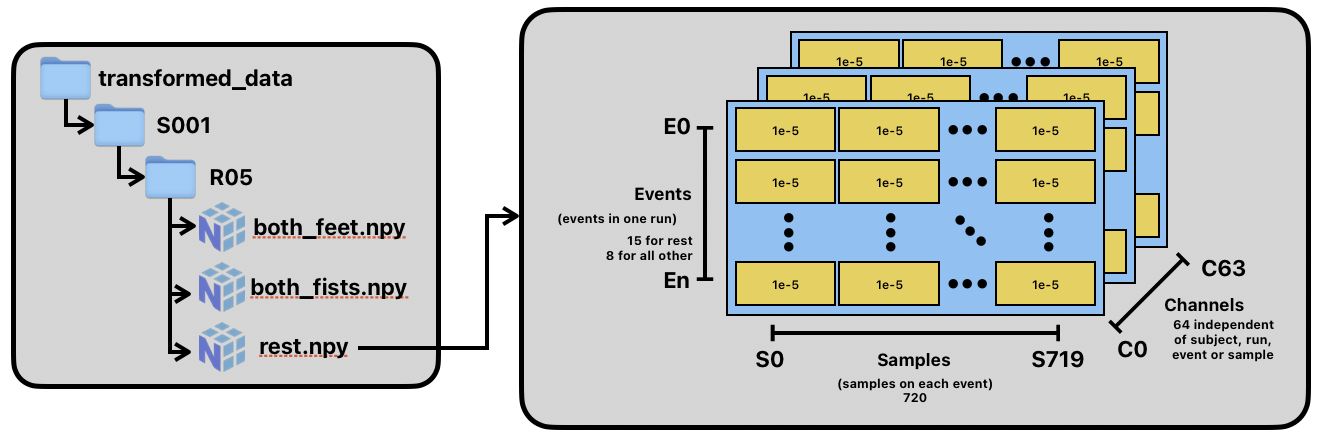
\includegraphics[width=1\linewidth]{assets/img/data_structure.png}
    \caption{Data structure after prepossessing}
    \label{fig:data-structure}
\end{figure}

\section{Initial Model Implementation}

An initial GRU model was implemented to begin the training process. Multiple runs were performed with default hyper-parameters to assess the model's performance.

\section{Data Tagging and DataLoader}

Tags were generated to match the sizes of each subject's events, ensuring correct classification. A DataLoader was implemented to shuffle the training data for model training.

\section{Data Transformation for Improved Training}

As the initial GRU model was not yielding satisfactory results, the following data transformations were made:

\begin{itemize}
    \item Events were flattened, consolidating them into a single dataset with 1800 events (10 subjects with 180 events each).
    \item Each event was transformed to have fewer GRU cells, joining samples together to achieve 10 cells with an input size of 4,608. See Fig. \ref{fig:joining_events_gru_cell}
    \begin{figure}[h]
        \centering
        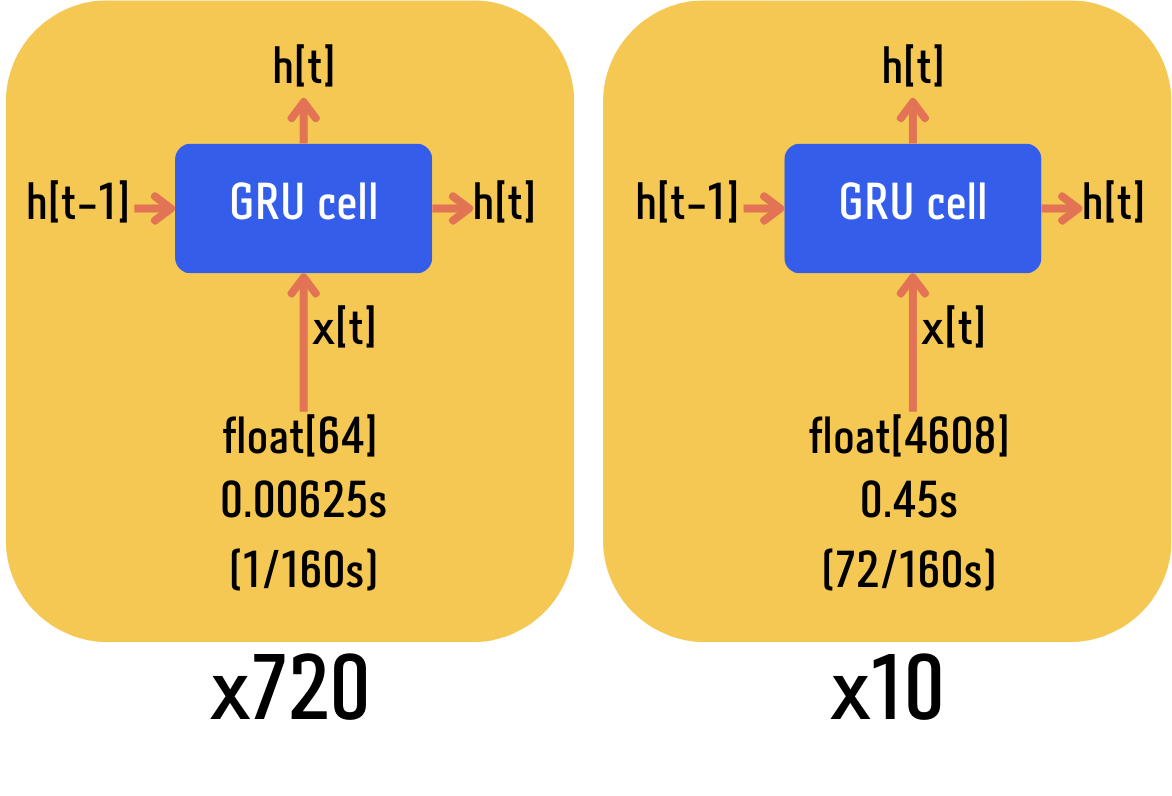
\includegraphics[width=0.5\linewidth]{assets/img/joining_events_gru_cell.png}
        \caption{Increase context for each GRU cell and reduce count of GRU cells. Before (left) and after (right)}
        \label{fig:joining_events_gru_cell}
    \end{figure}
\end{itemize}


\section{In-Depth Analysis}

Despite the above changes, the model's accuracy remained low, and in-depth analysis was conducted:

\begin{itemize}
    \item Data was reviewed to identify anomalies, but none were found.
    \item The problem was reduced to comparing events of a single subject, which should theoretically yield better results. However, accuracy remained below random guessing (50%).
\end{itemize}

\section{Reducing Noise through Channel Selection}

Upon consultation with thesis advisor, Jose Antonio Cantoral-Ceballos, Ph.D., the following change was implemented to reduce noise in the system:

\begin{itemize}
    \item A selection of the central group of 9 nodes (FC[1, Z, 2], C[1, Z, 2], CP[1, Z, 2]) was made. See Fig. \ref{fig:eeg_channel_selection}
    \begin{figure}[h]
        \centering
        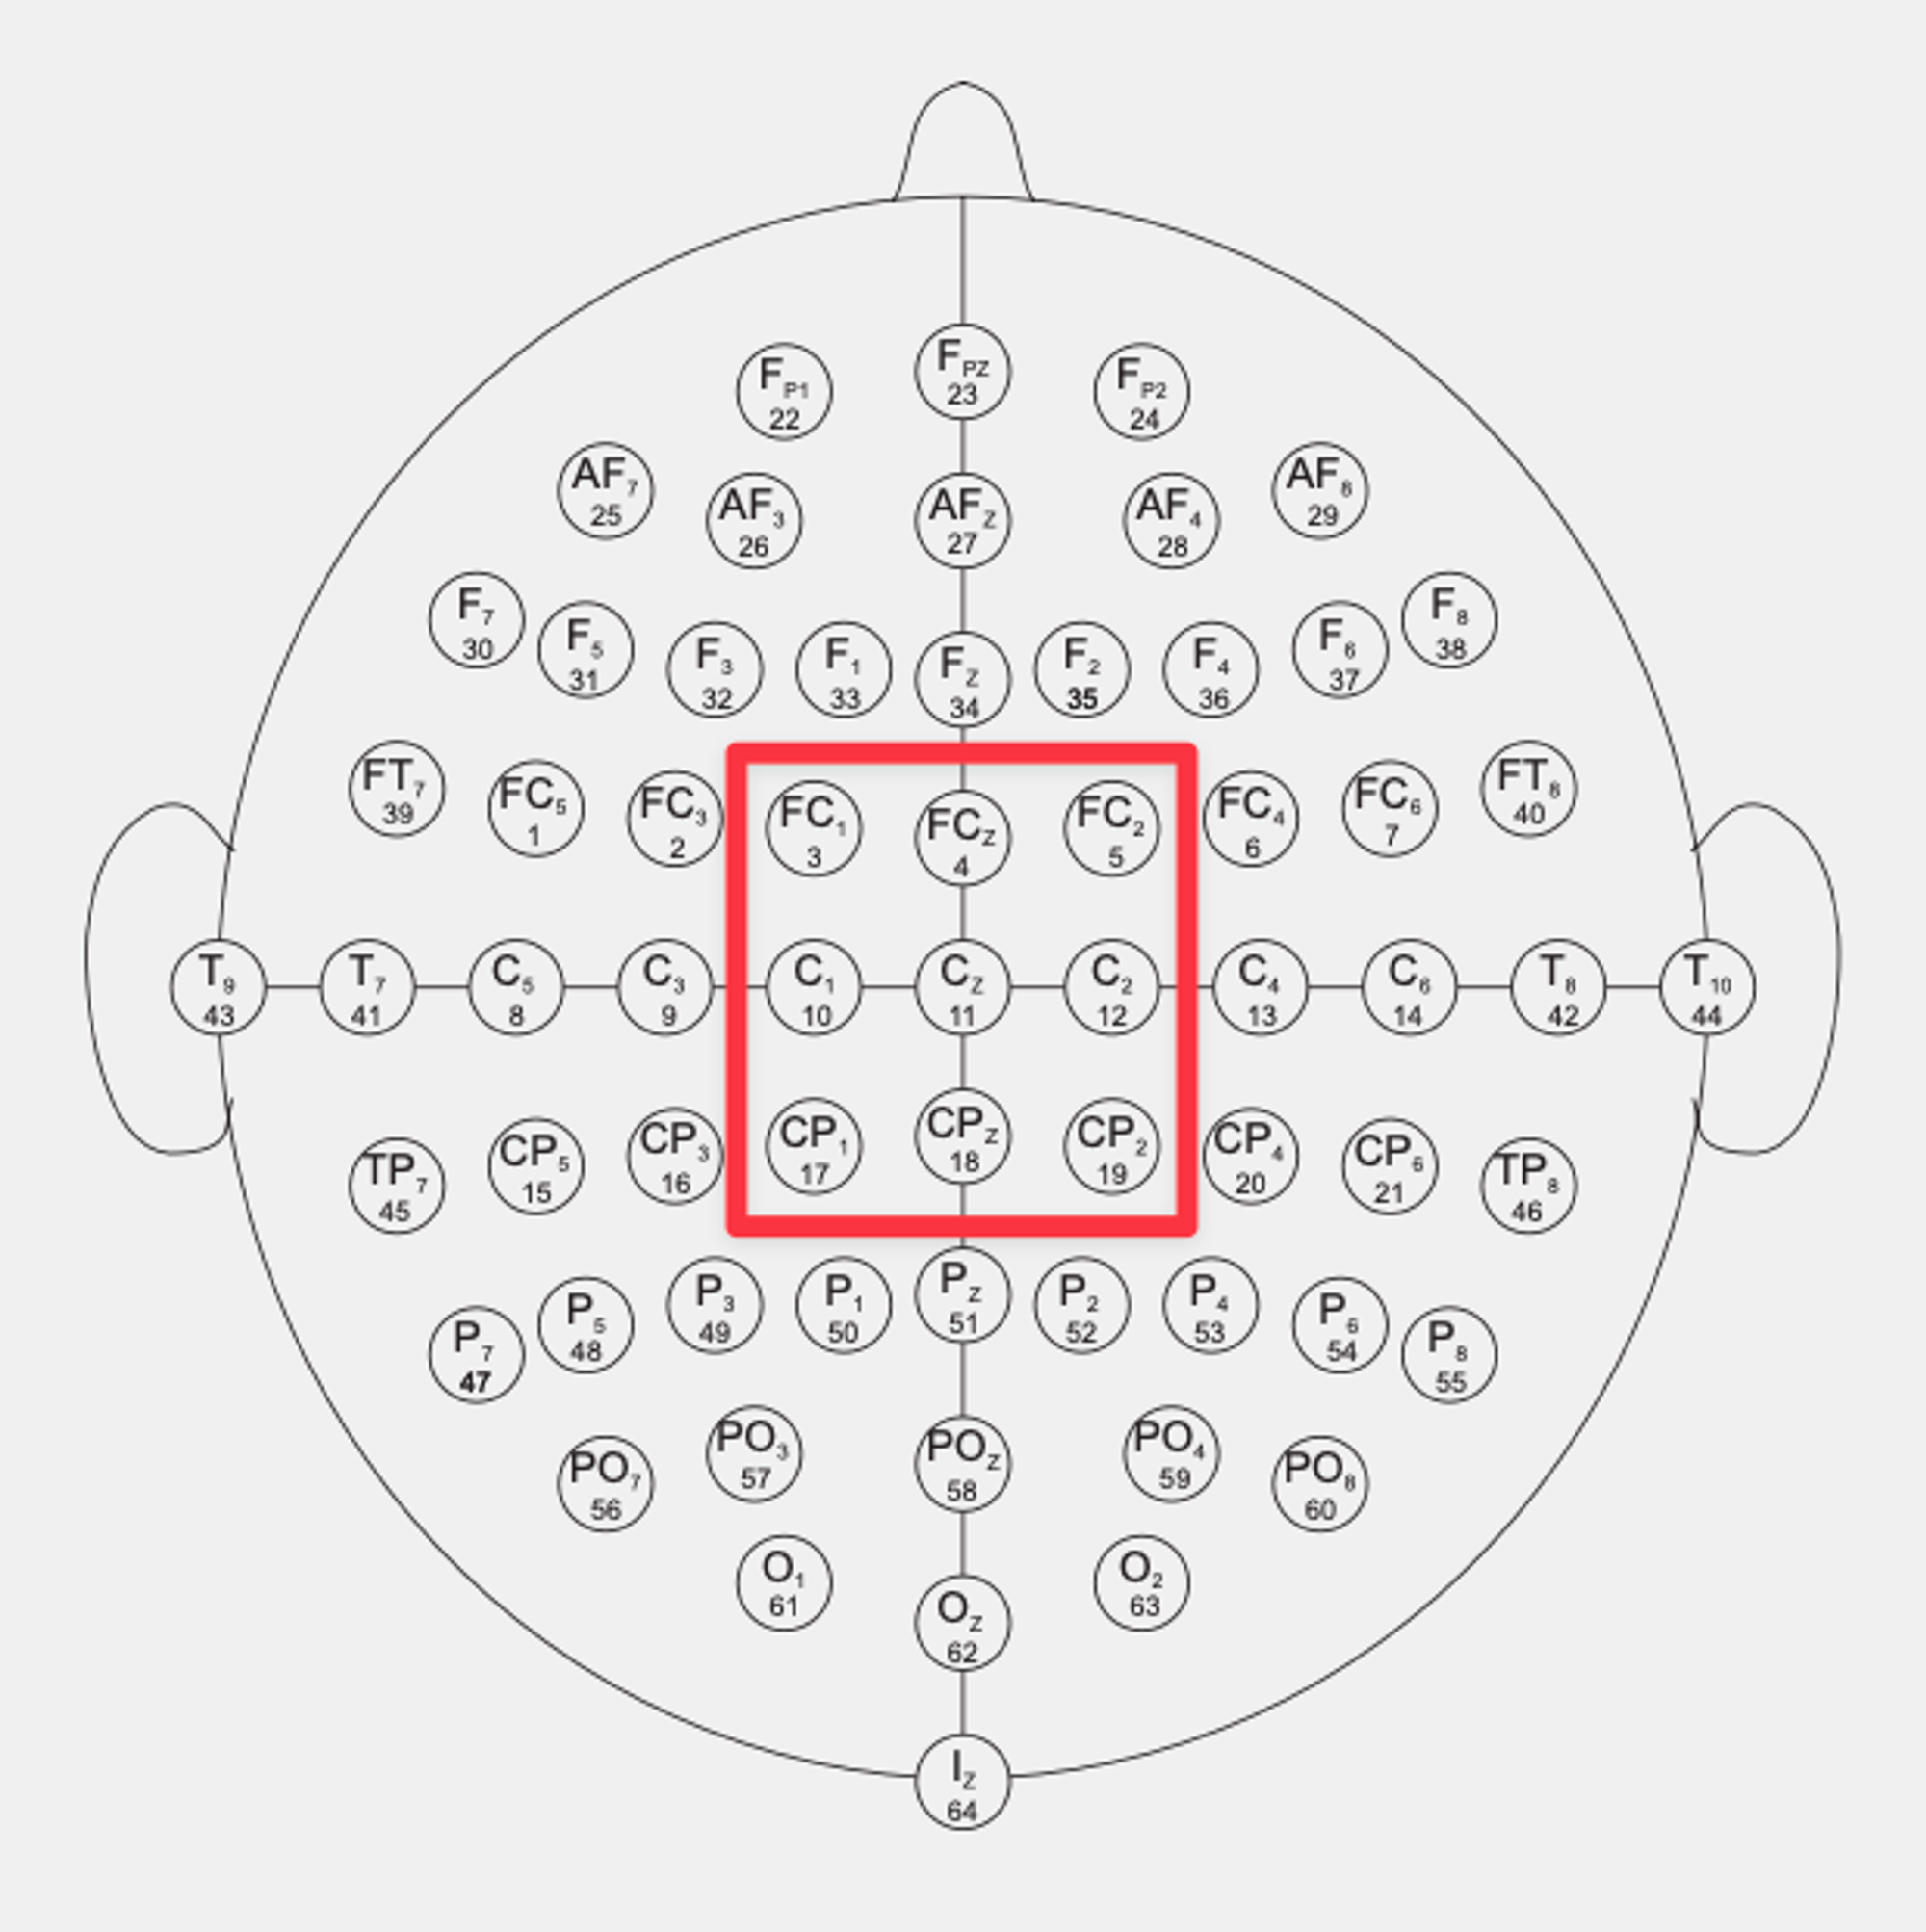
\includegraphics[width=0.5\linewidth]{assets/img/eeg_channel_selection.png}
        \caption{Graphic shows all available EEG channels. Red square indicates selection of selected central nodes}
        \label{fig:eeg_channel_selection}
    \end{figure}
\end{itemize}

\section{Model Fine-Tuning}

Additional tests were conducted with the modified dataset and GRU model:

\begin{itemize}
    \item Different LRs were tested to find optimal option to train with. The best LRs in training showed to be 1e-2, 8e-3 and 5e-3 asn shown on Fig. \ref{fig:fine_tuning_lr}\\
    \begin{figure}[h]
        \centering
        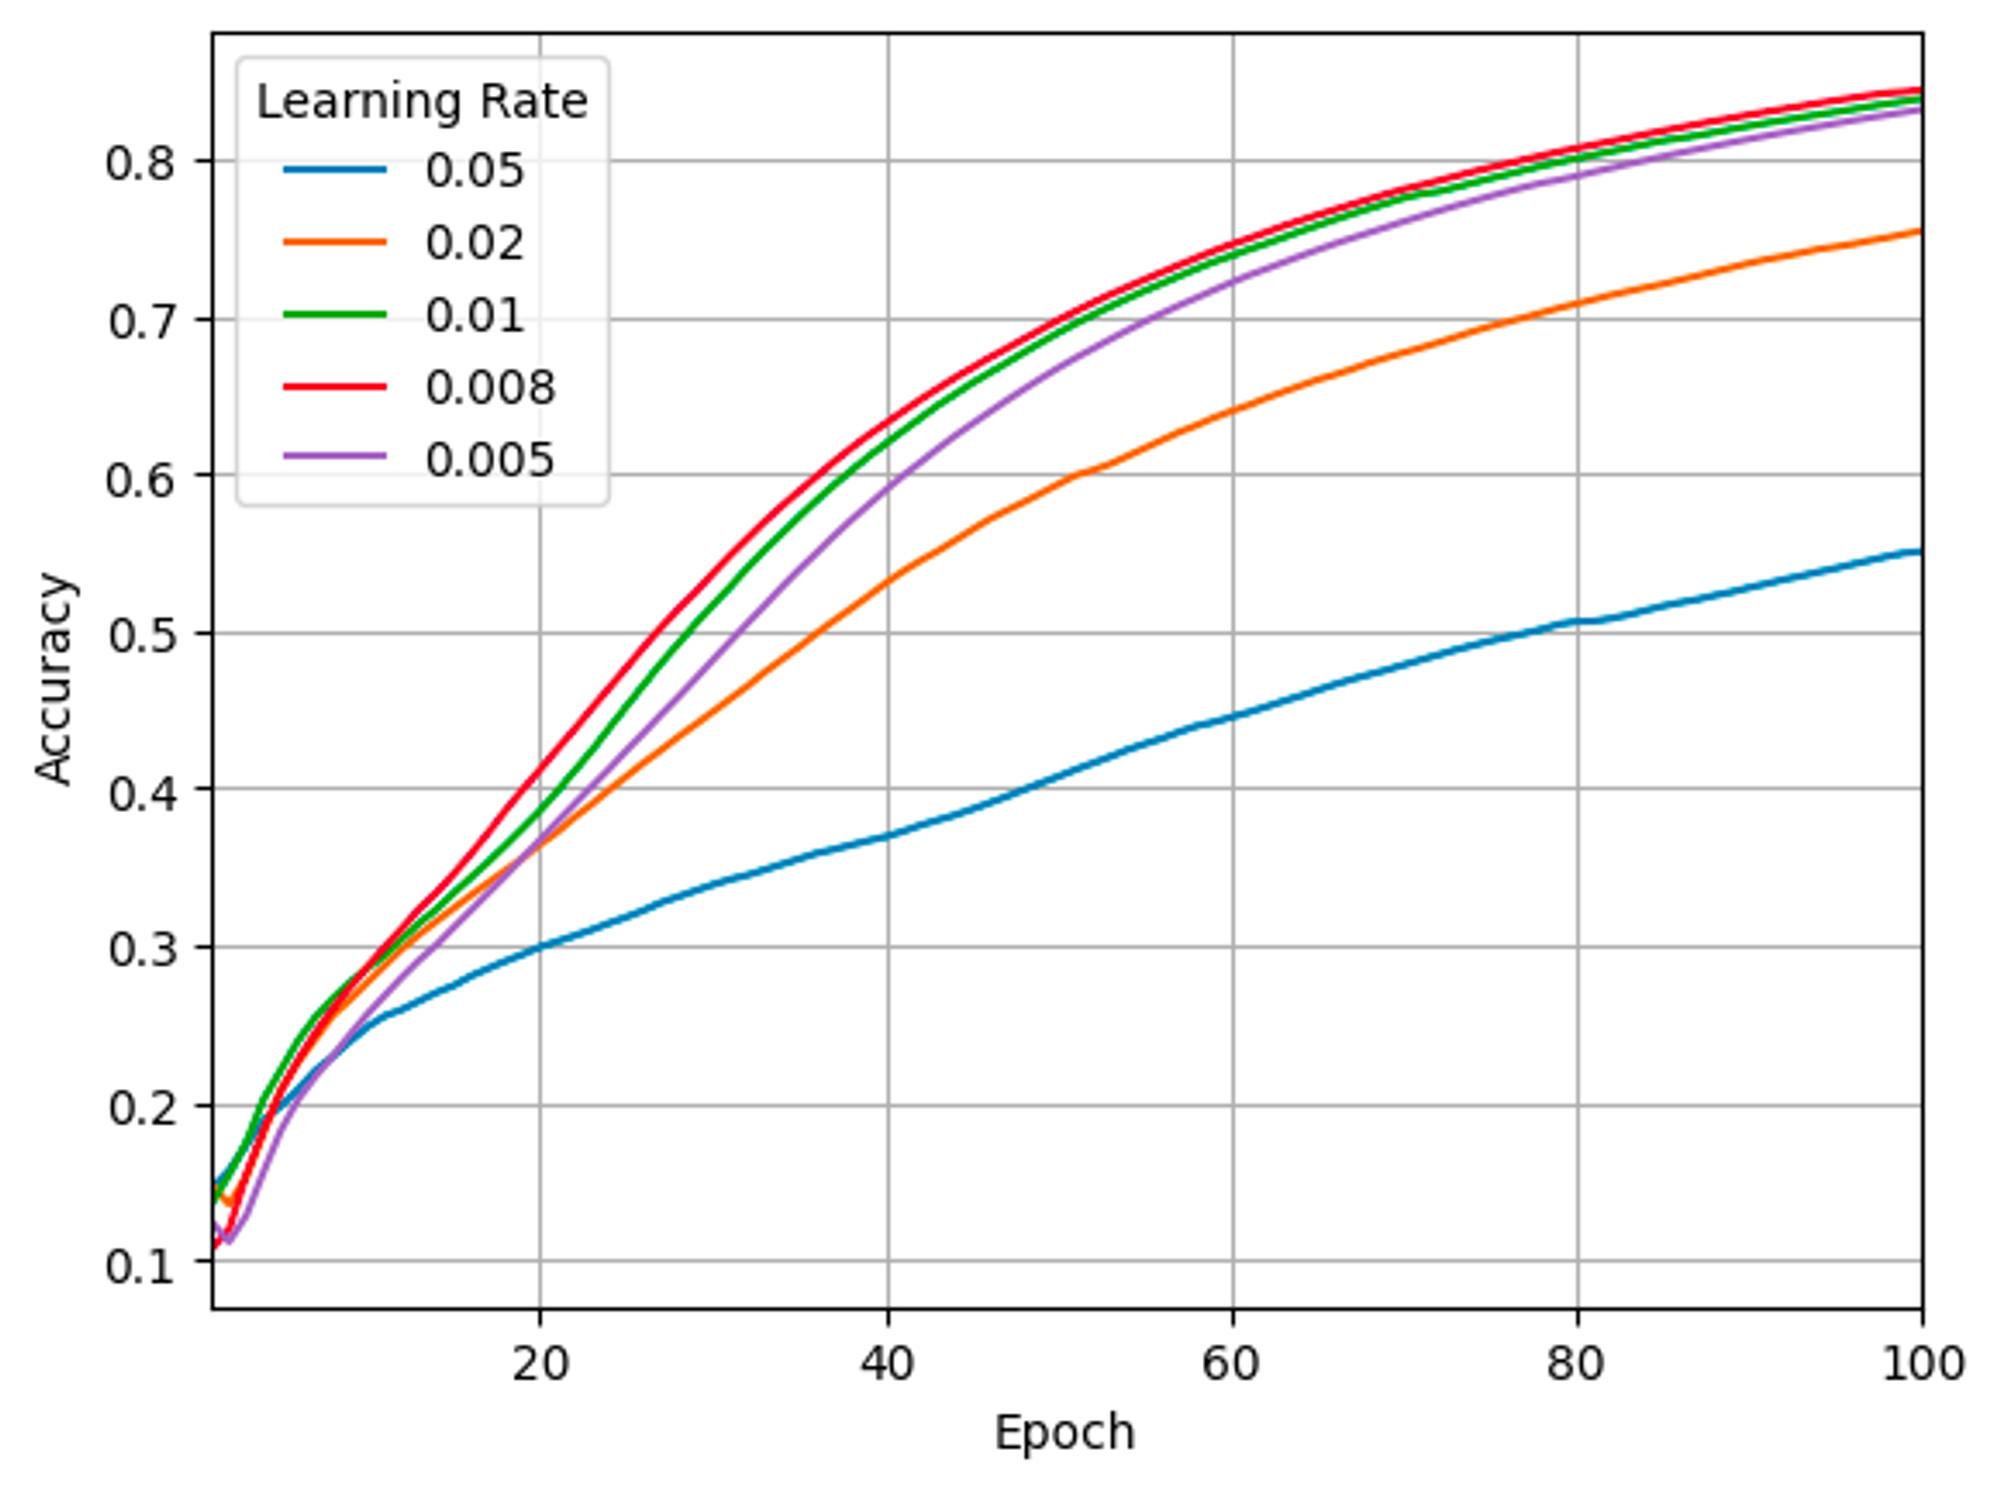
\includegraphics[width=0.7\linewidth]{assets/img/fine_tuning_lr.png}
        \caption{}
        \label{fig:fine_tuning_lr}
    \end{figure}
    
    Later with a test sample these yielded the following accuracies:
    \begin{itemize} 
        \item 1e-2 → 62.3%
        \item 8e-3 → 54.7%
        \item 5e-3 → 54.5%
    \end{itemize}

    \item Implementing OneCycleLR scheduler \cite{smith2018superconvergence} with various values was tested and showed small but consistent positive results of +5\% in test accuracy (Figs. \ref{fig:onecycle_stable_lr} and \ref{fig:onecycle_decreasing_lr}).
    
    \begin{figure}[h]
        \centering
        \begin{subfigure}[b]{0.5\textwidth}
            \centering
            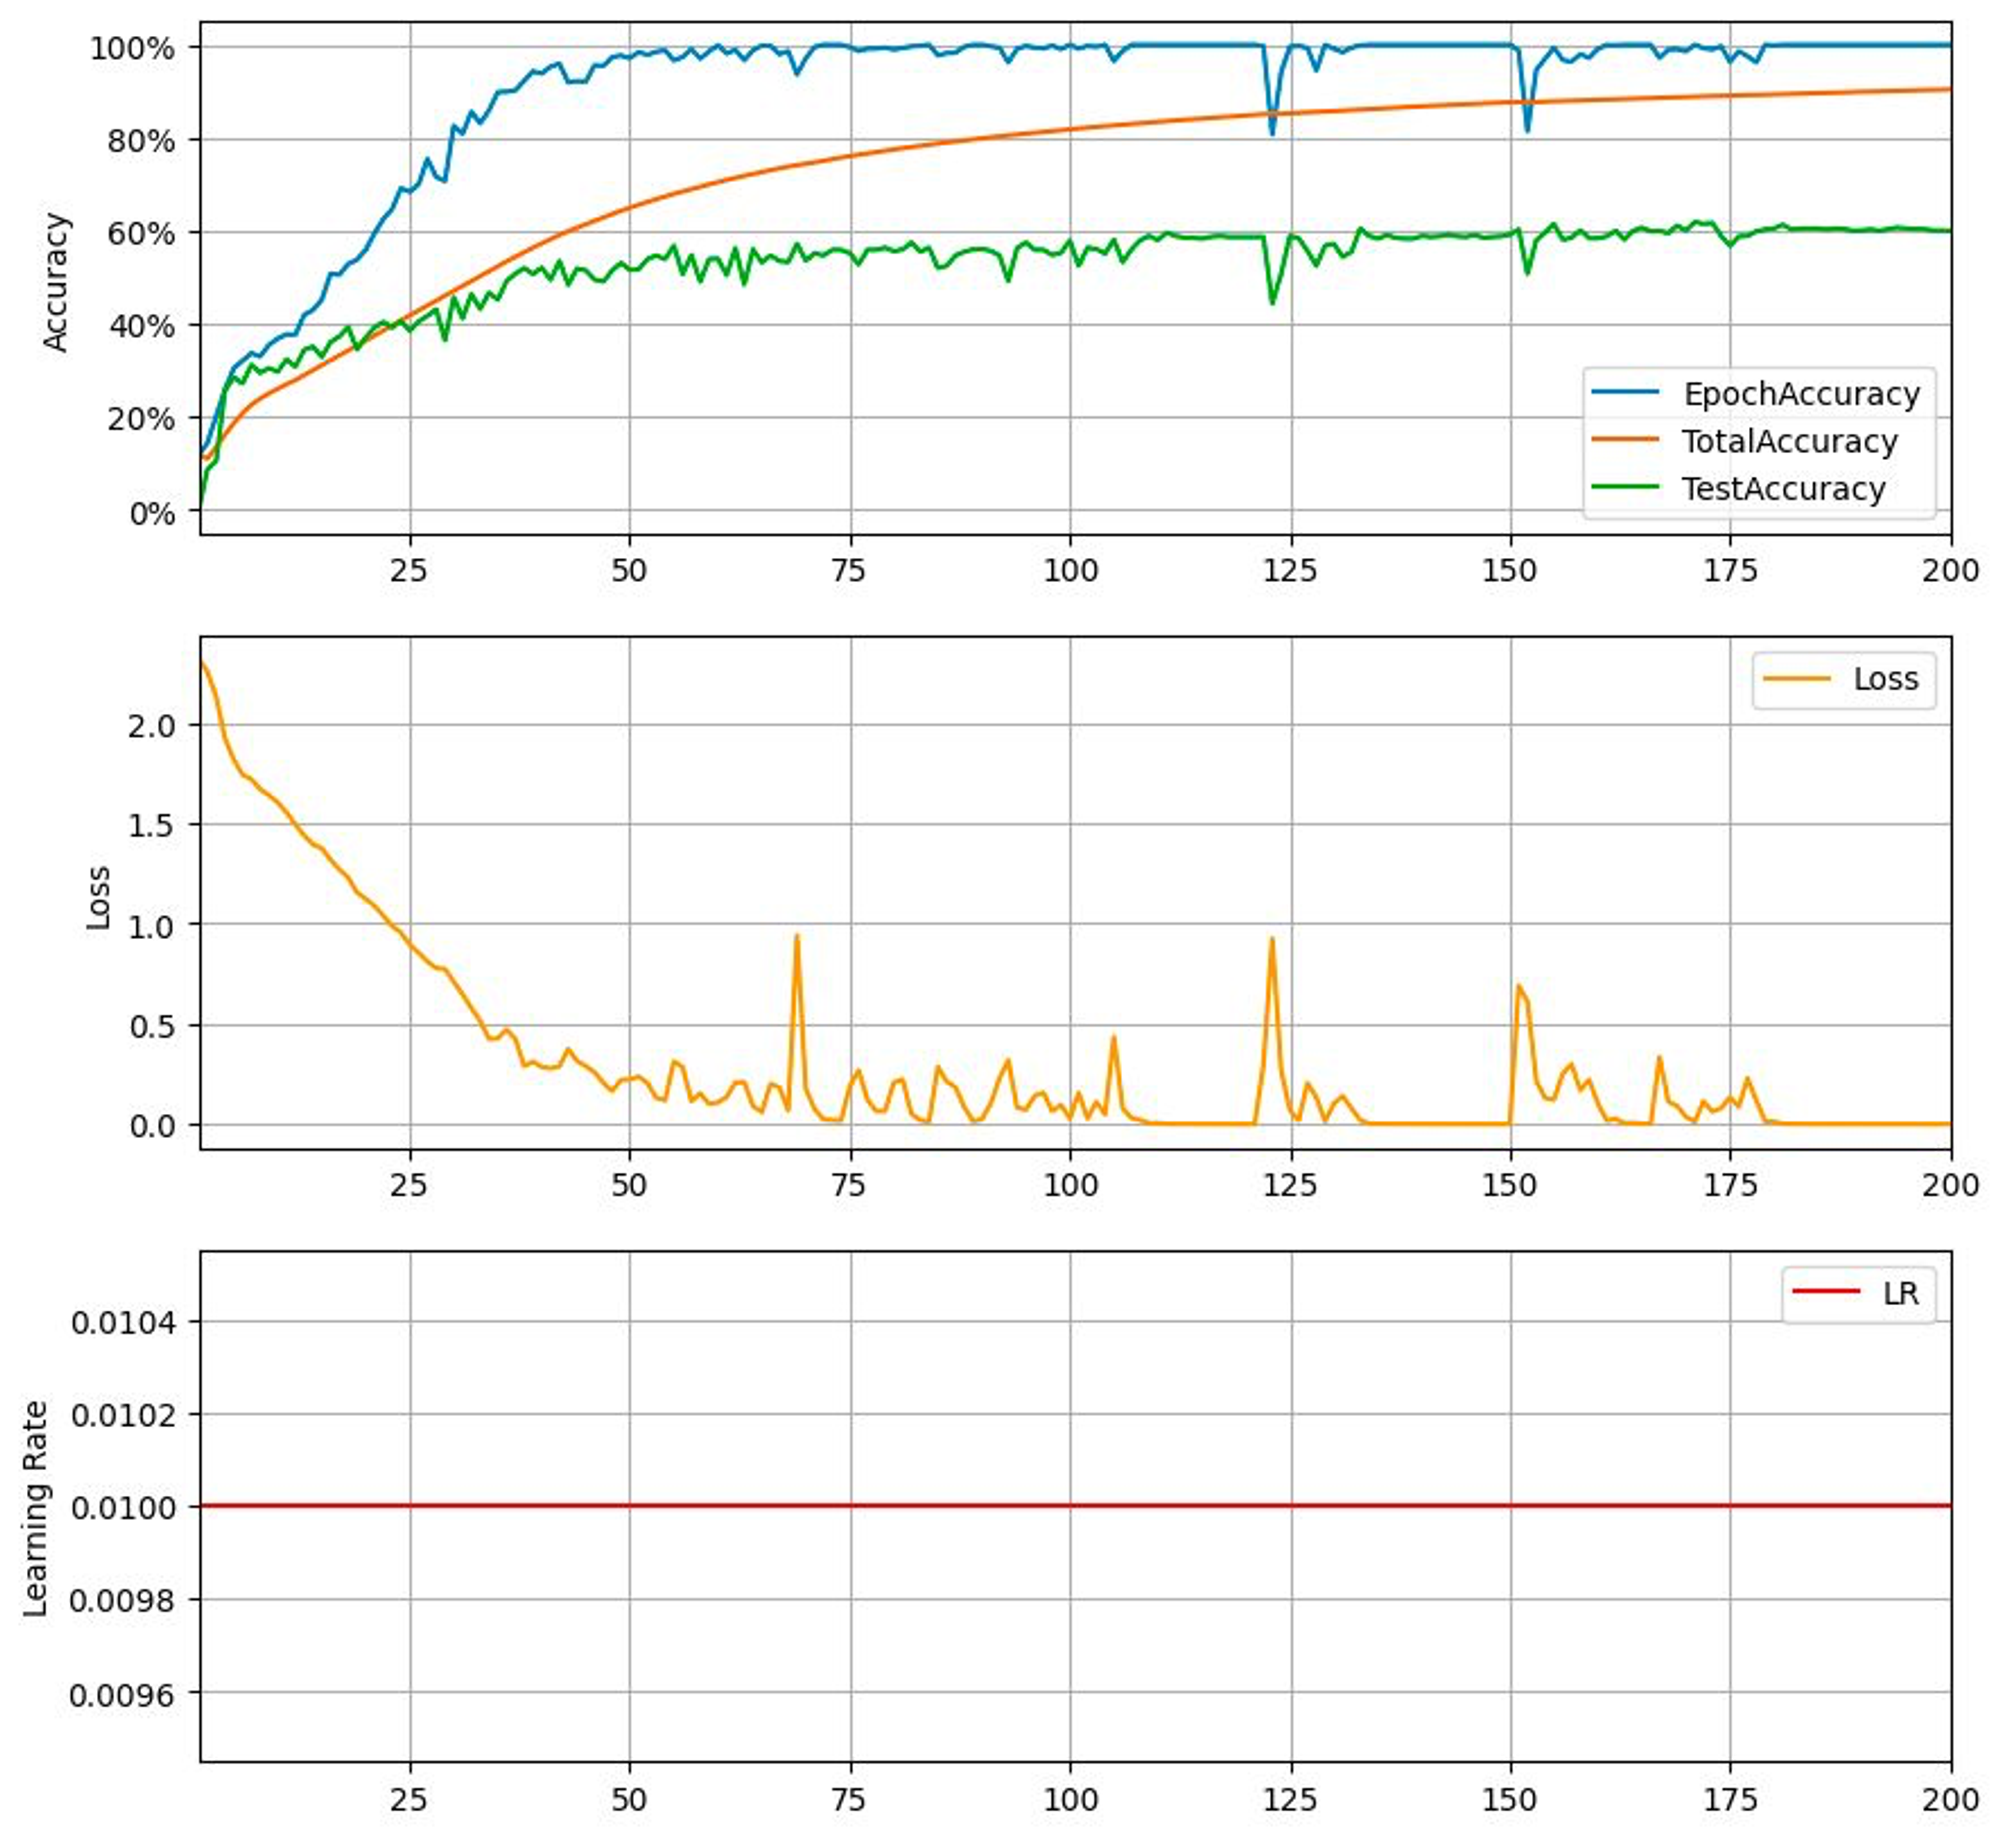
\includegraphics[width=\textwidth]{assets/img/onecycle_stable_lr.png}
            \caption{[1e-2, 1e-4]}
            \label{fig:onecycle_stable_lr}
        \end{subfigure}%
        \hfill
        \begin{subfigure}[b]{0.5\textwidth}
            \centering
            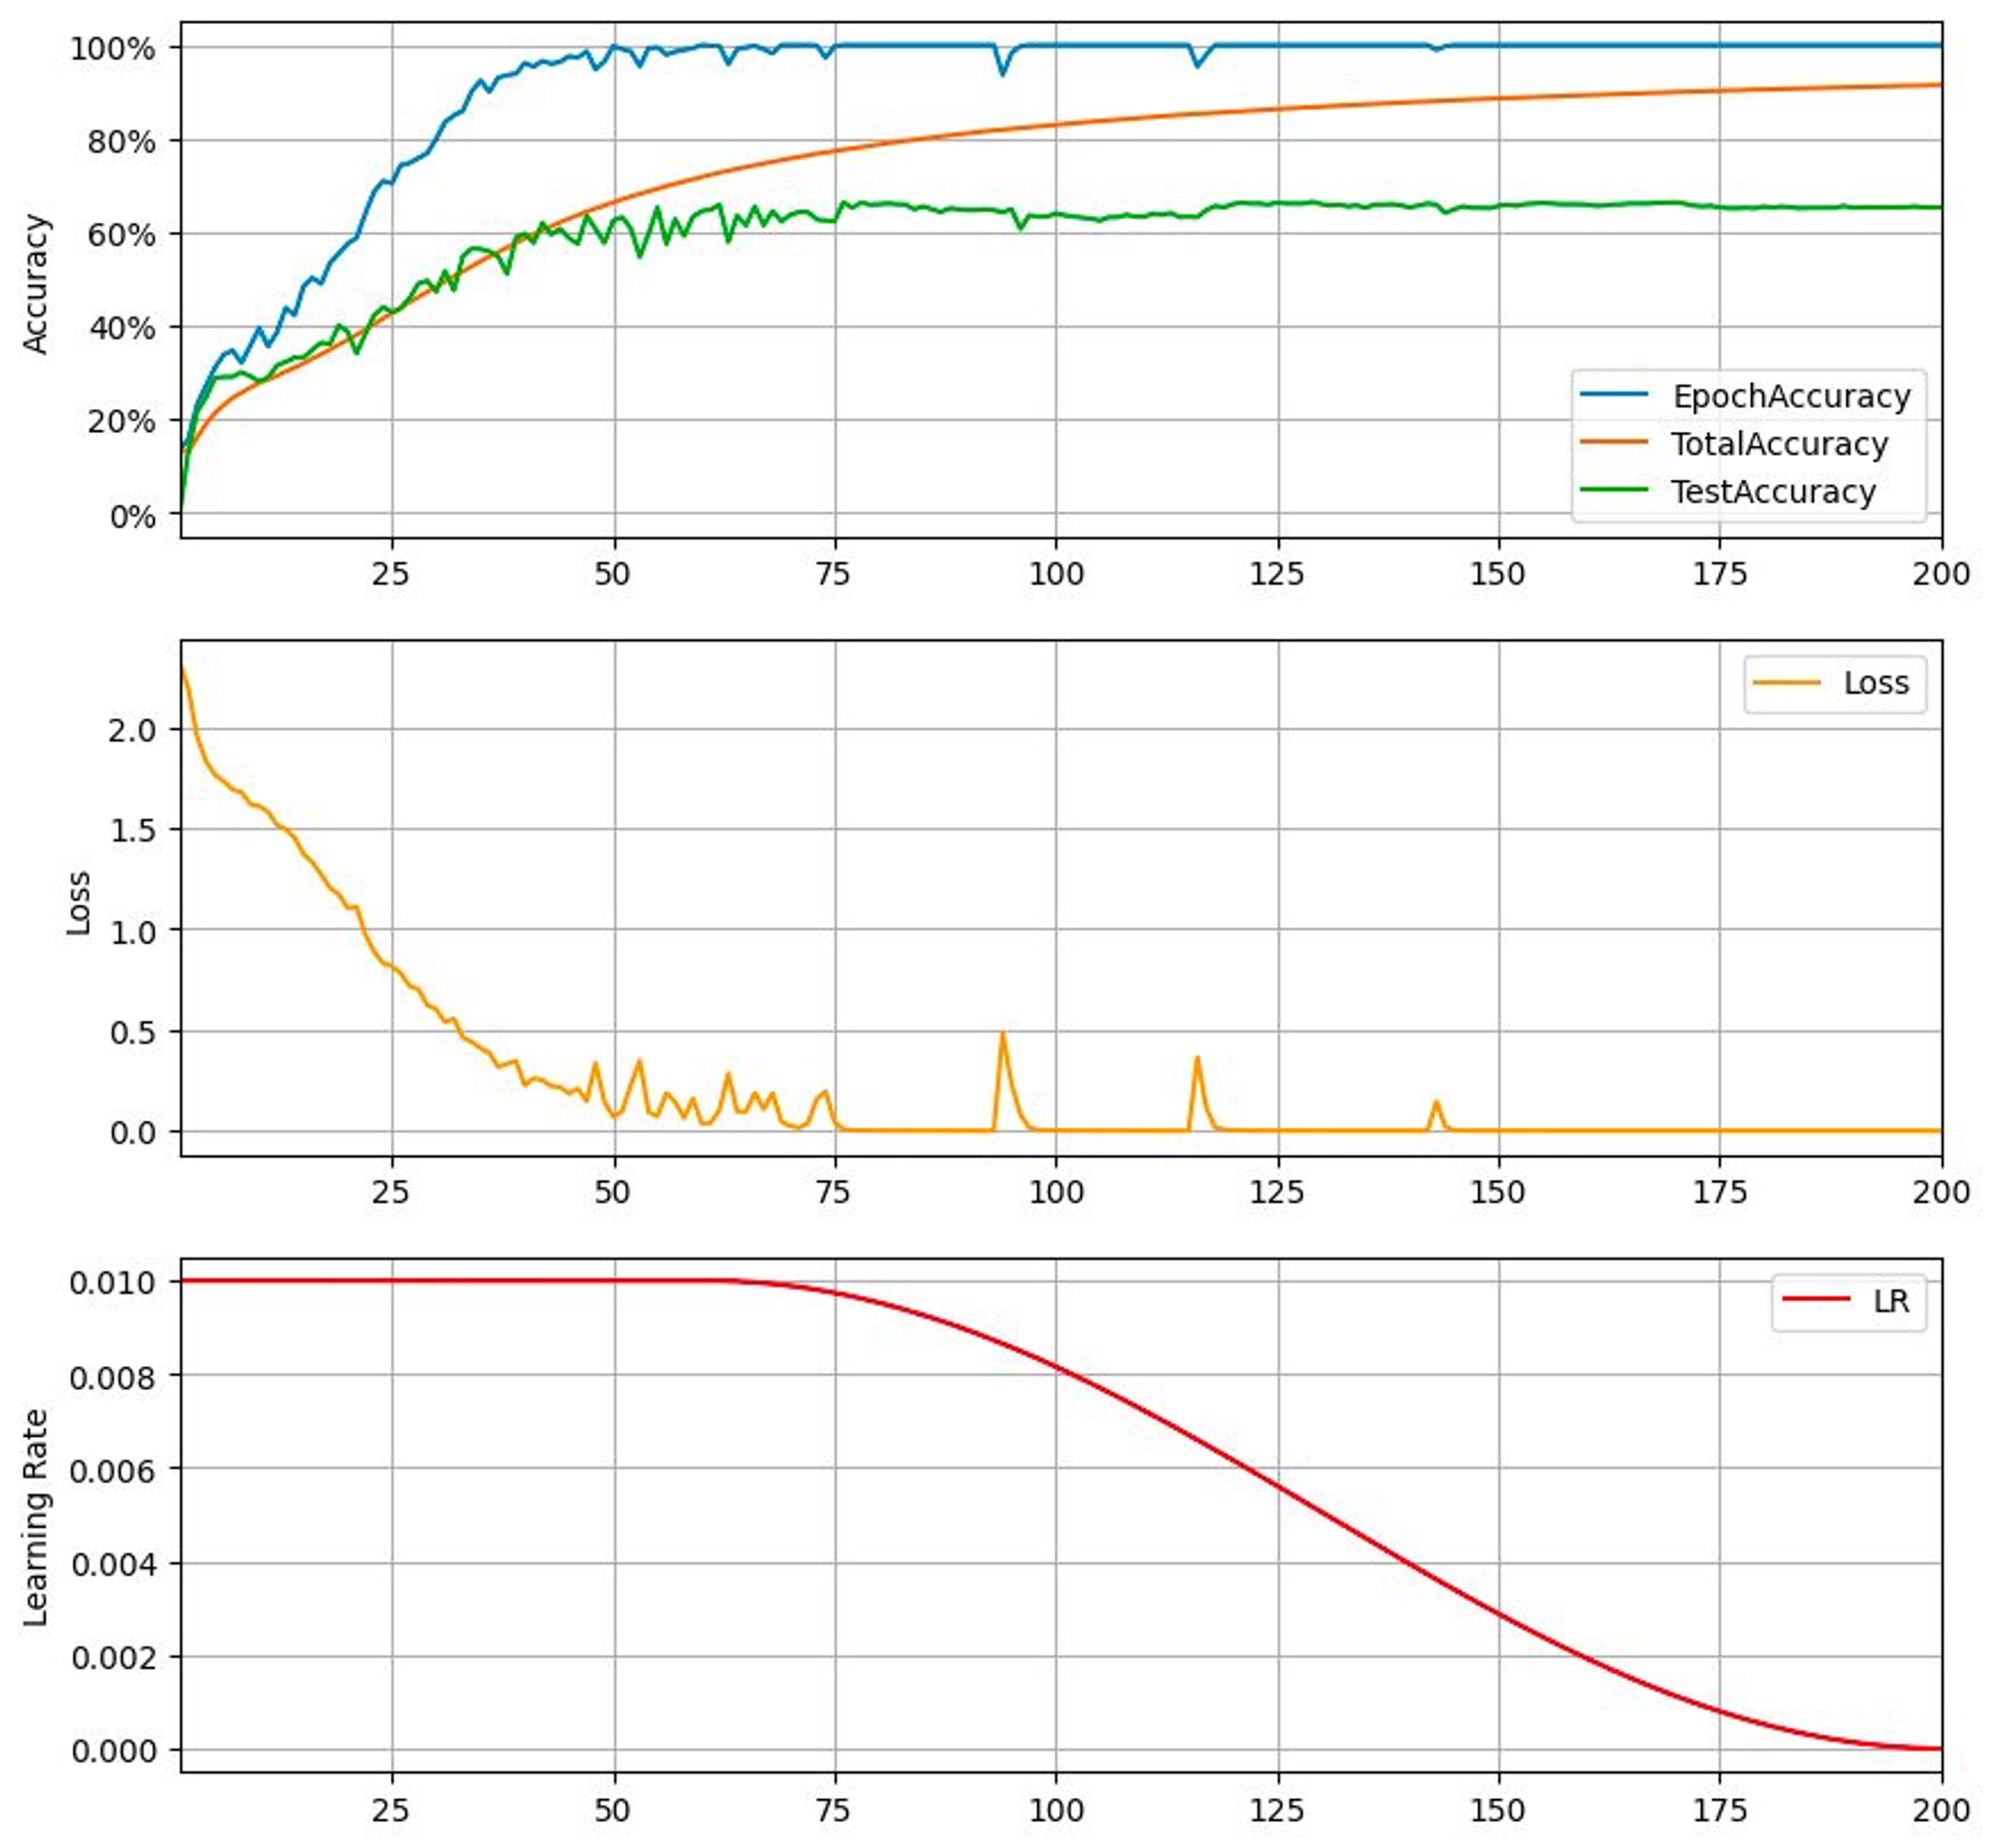
\includegraphics[width=\textwidth]{assets/img/onecycle_decreasing_lr.png}
            \caption{[1e-2]}
            \label{fig:onecycle_decreasing_lr}
        \end{subfigure}%
        \caption{OneCycleLR comparisons}
    \end{figure}

    \item Finding an appropiate Label Smoothing in the Cross entropy loss function \cite{szegedy2015rethinking}. This showed a big increase in test accuracy (From 40\% to 80\%) (Figs. \ref{fig:label_smoothing_total} and \ref{fig:label_smoothing_test})
    \begin{figure}[h]
        \centering
        \begin{subfigure}[b]{0.5\textwidth}
            \centering
            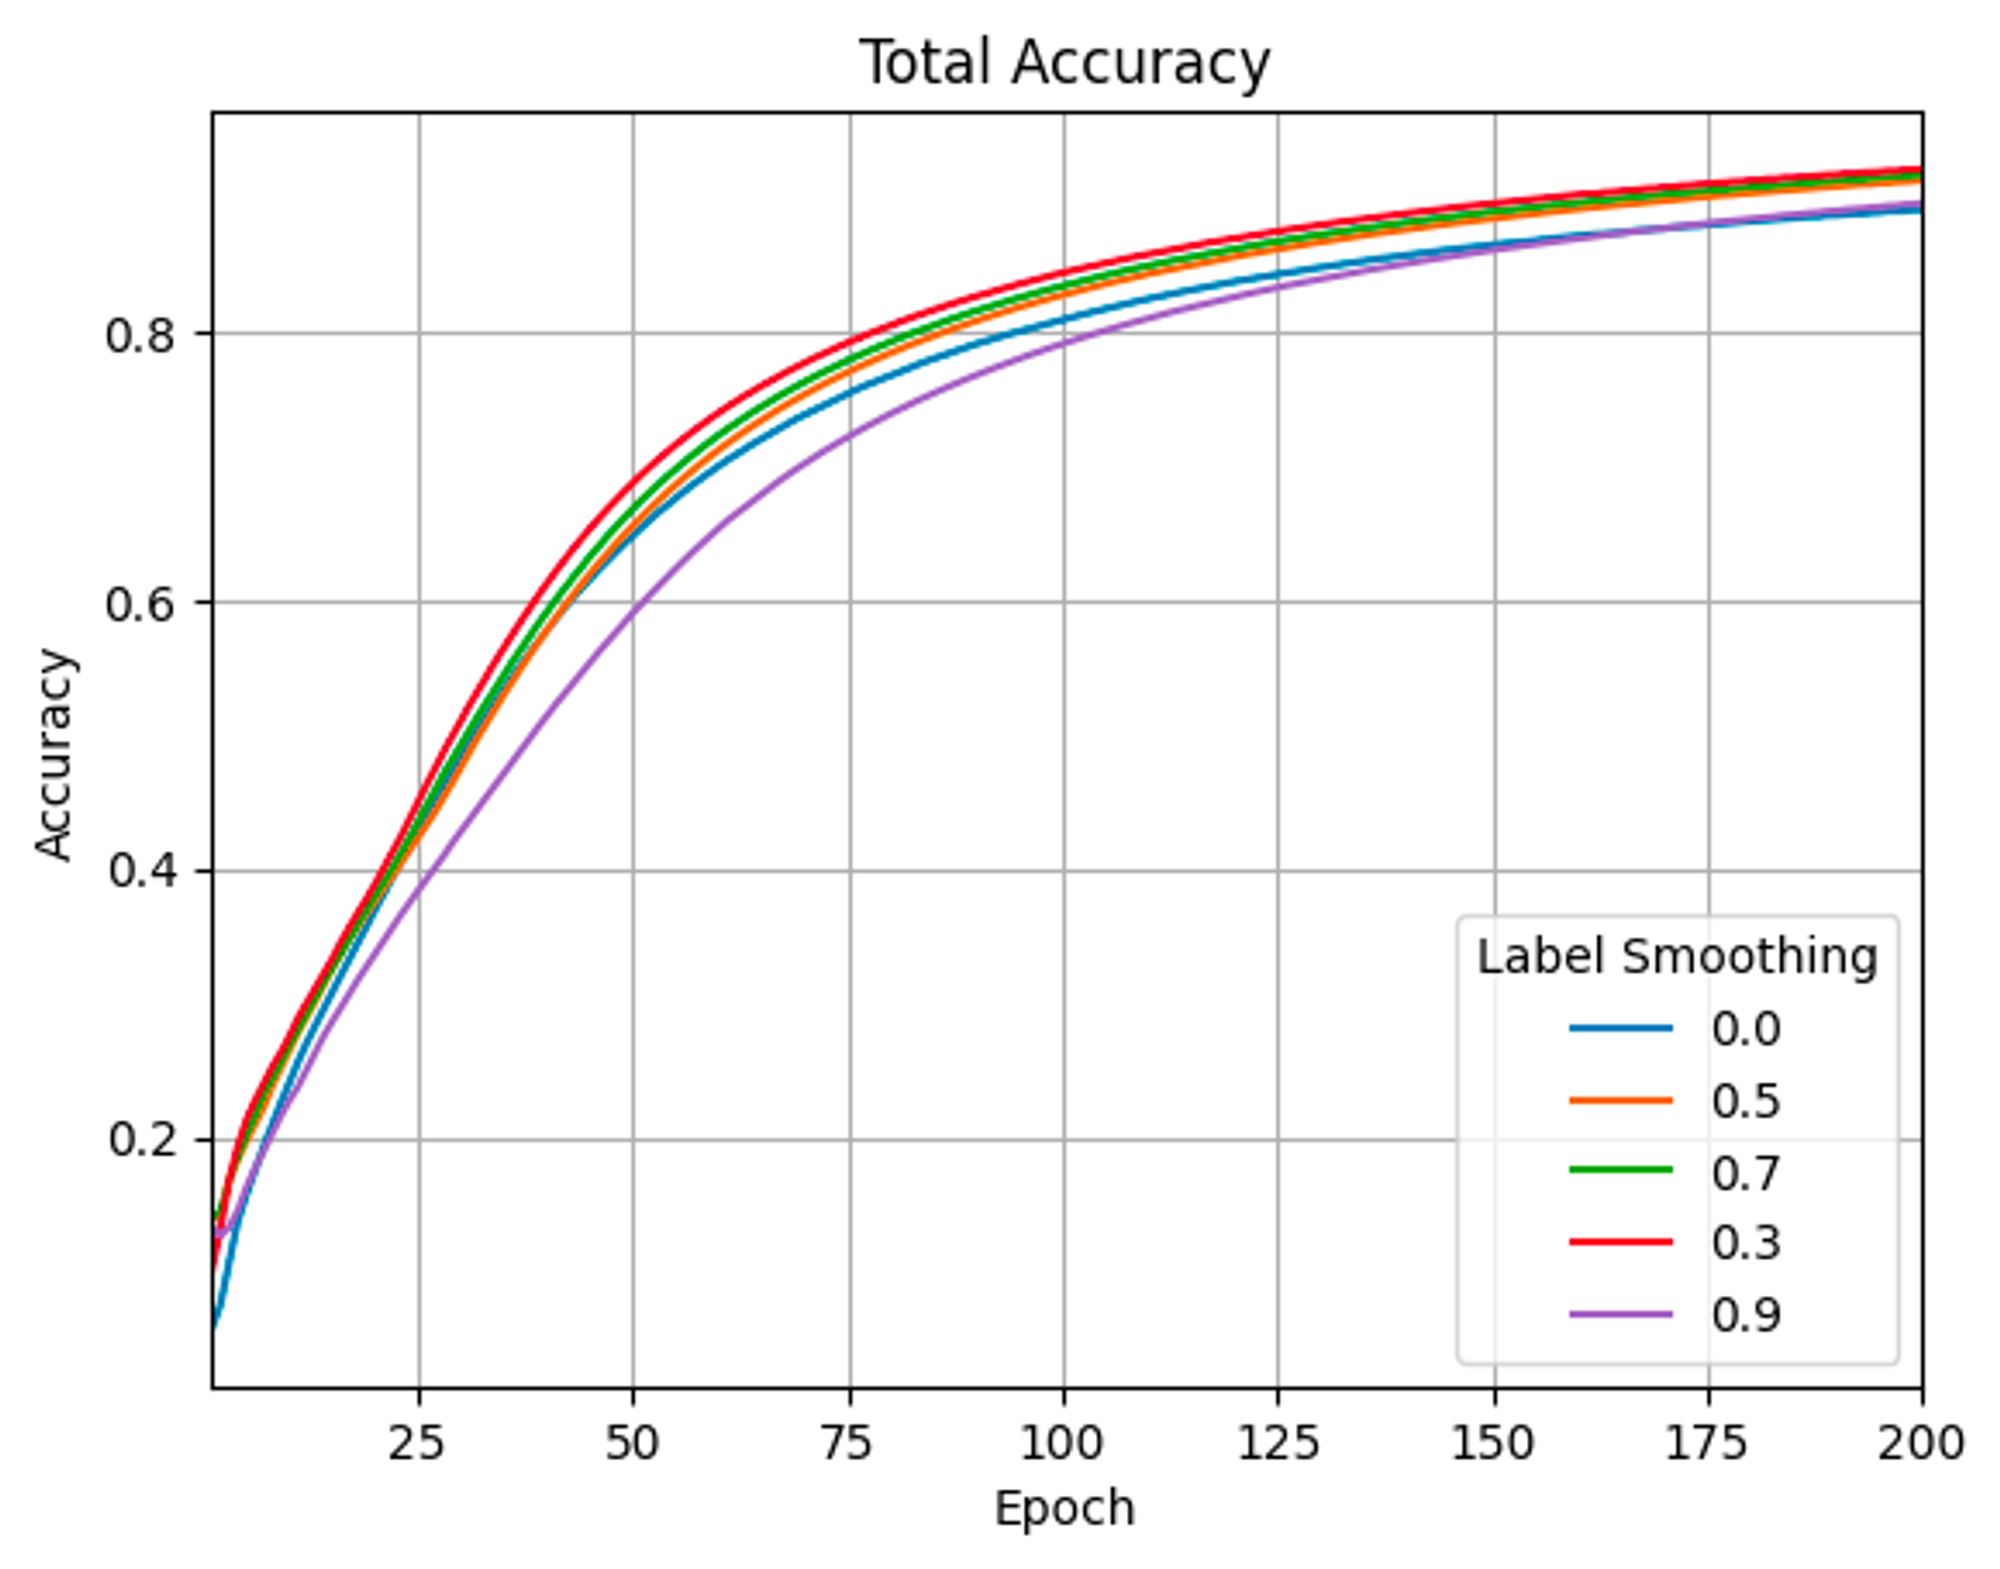
\includegraphics[width=\textwidth]{assets/img/label_smoothing_total.png}
            \caption{Training accuracy}
            \label{fig:label_smoothing_total}
        \end{subfigure}%
        \hfill
        \begin{subfigure}[b]{0.5\textwidth}
            \centering
            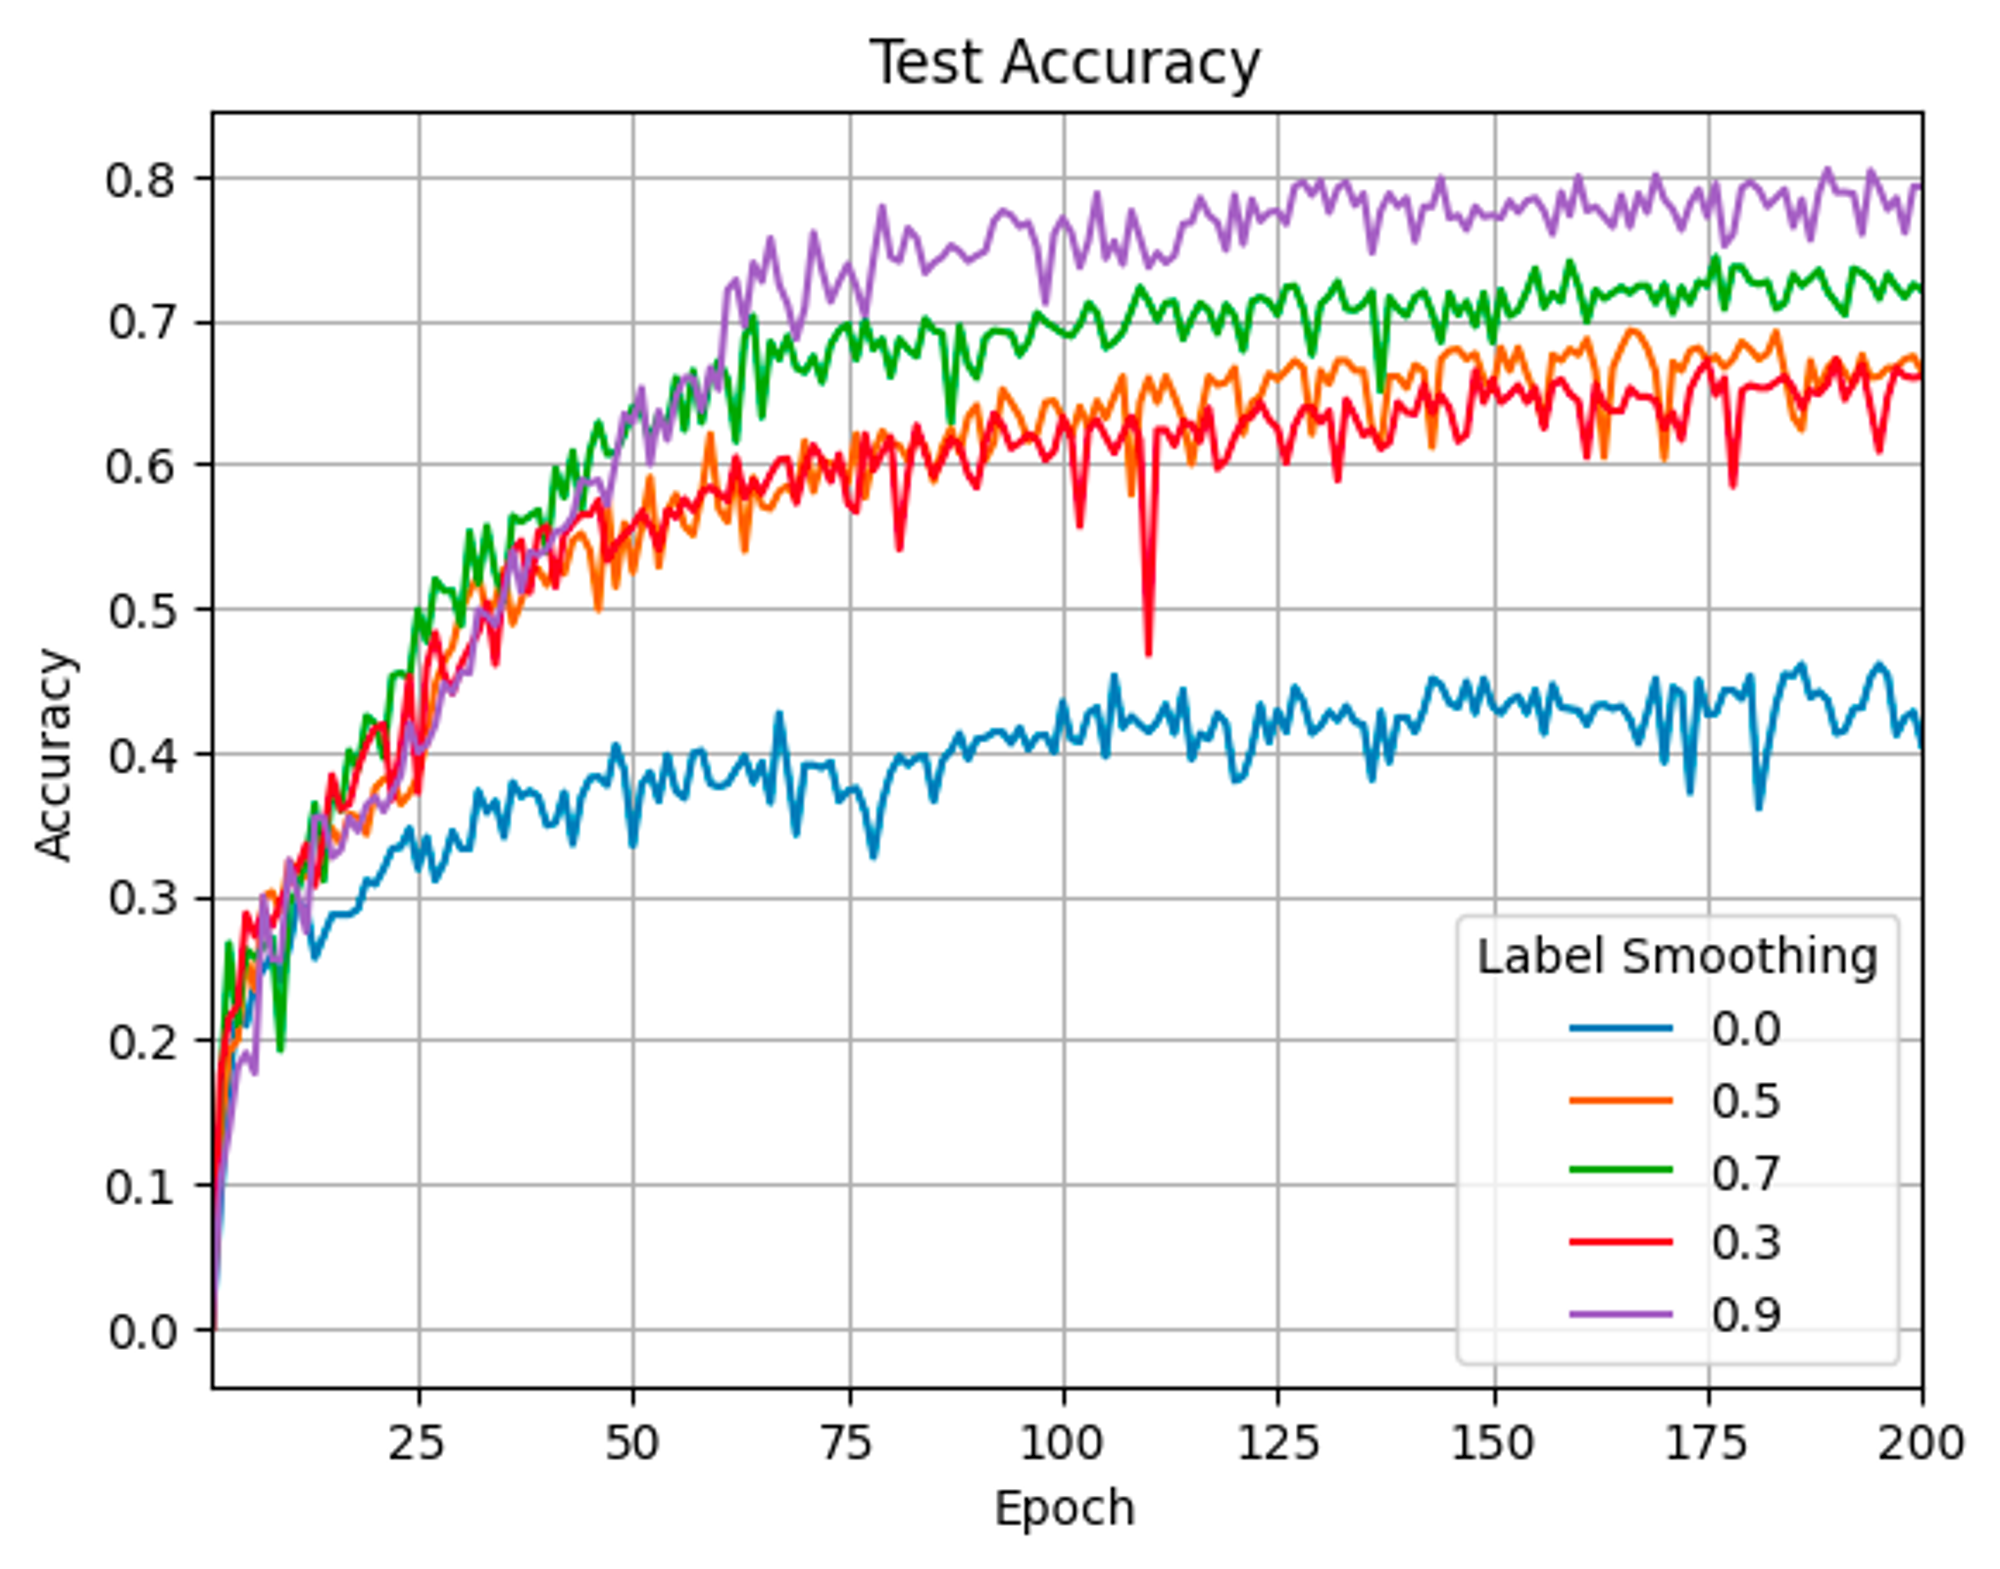
\includegraphics[width=\textwidth]{assets/img/label_smoothing_test.png}
            \caption{Test accuracy}
            \label{fig:label_smoothing_test}
        \end{subfigure}%
        \caption{Runs with various values of label smoothing}
    \end{figure}

    \item Joining OneCycleLR and Label Smoothing and testing with various parameters to find the best output. (Figs. \ref{fig:onecycle_tests_lr}, \ref{fig:onecycle_tests_train_acc}, \ref{fig:onecycle_tests_test_acc})

    \begin{figure}[h]
        \centering
        \begin{subfigure}[b]{0.3\textwidth}
            \centering
            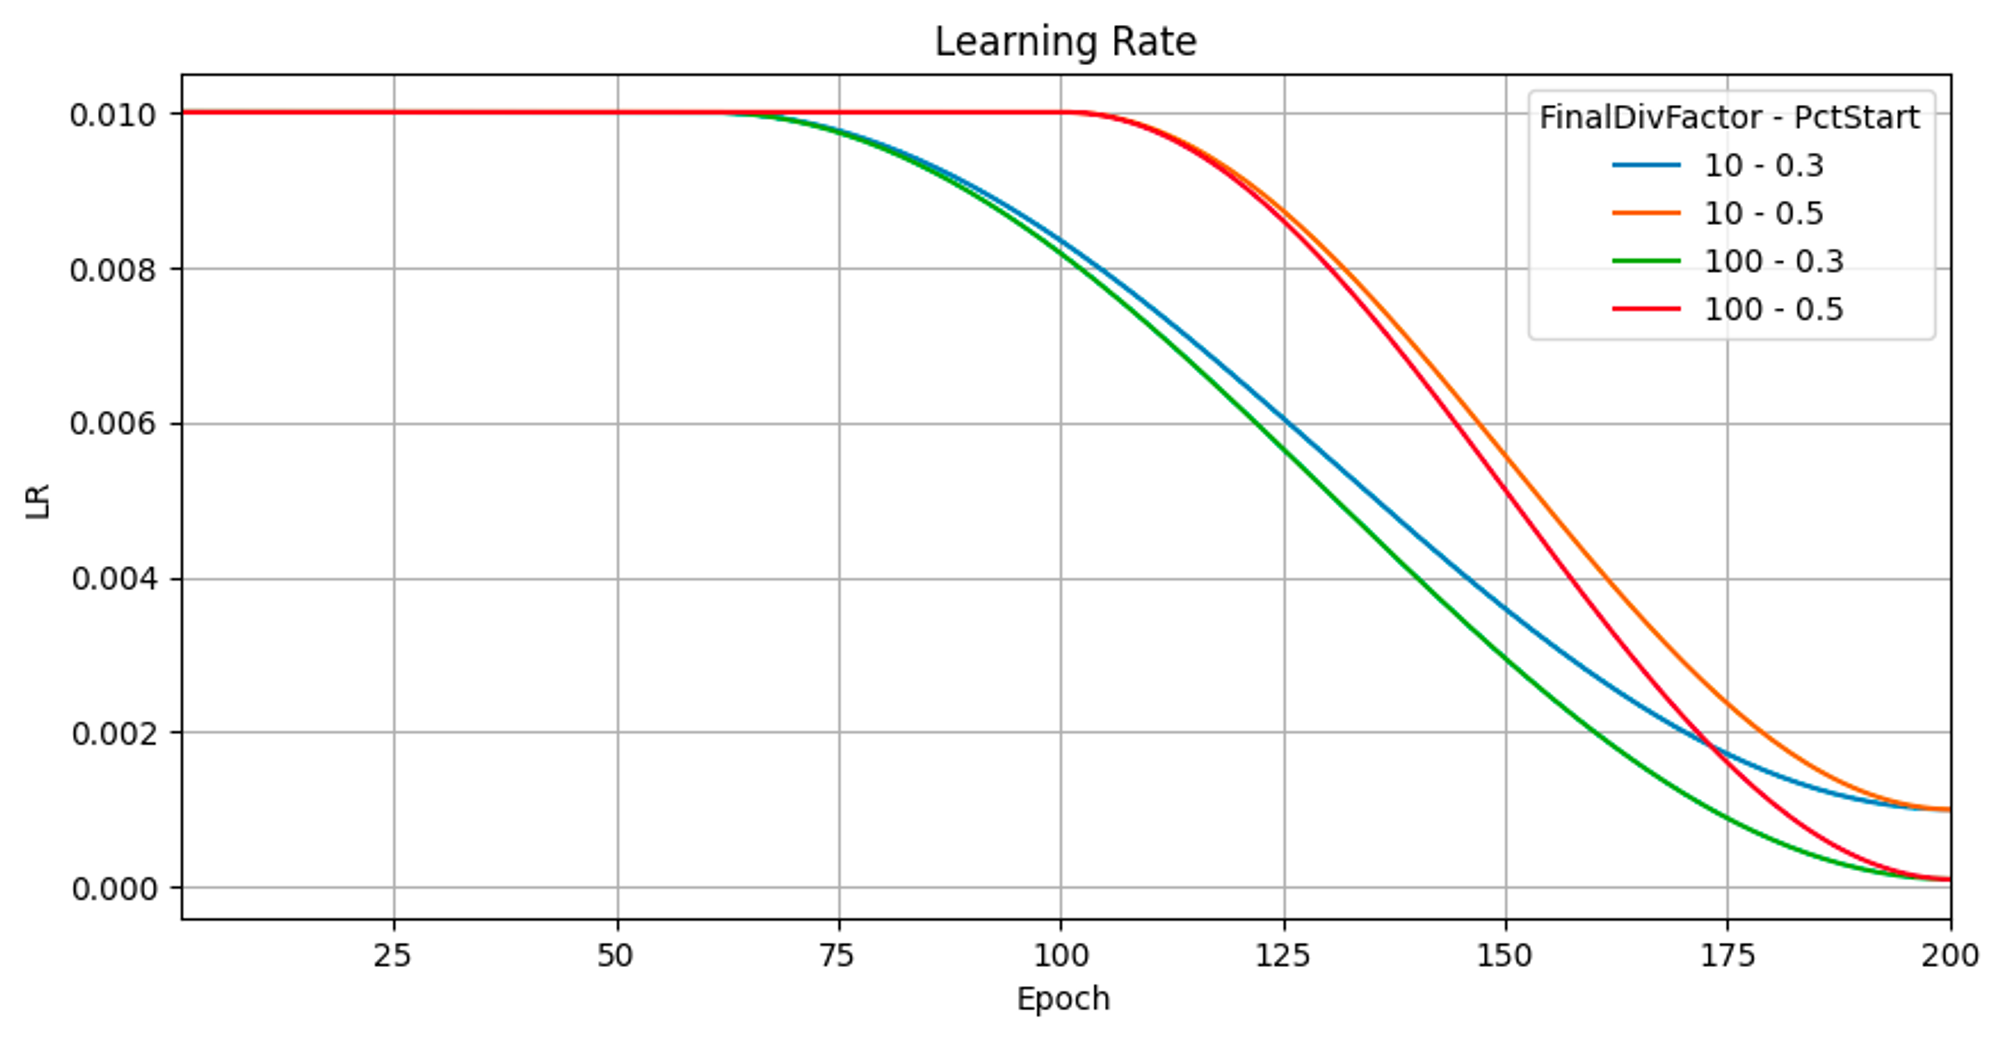
\includegraphics[width=\textwidth]{assets/img/onecycle_tests_lr.png}
            \caption{LR evolution}
            \label{fig:onecycle_tests_lr}
        \end{subfigure}%
        \hfill
        \begin{subfigure}[b]{0.3\textwidth}
            \centering
            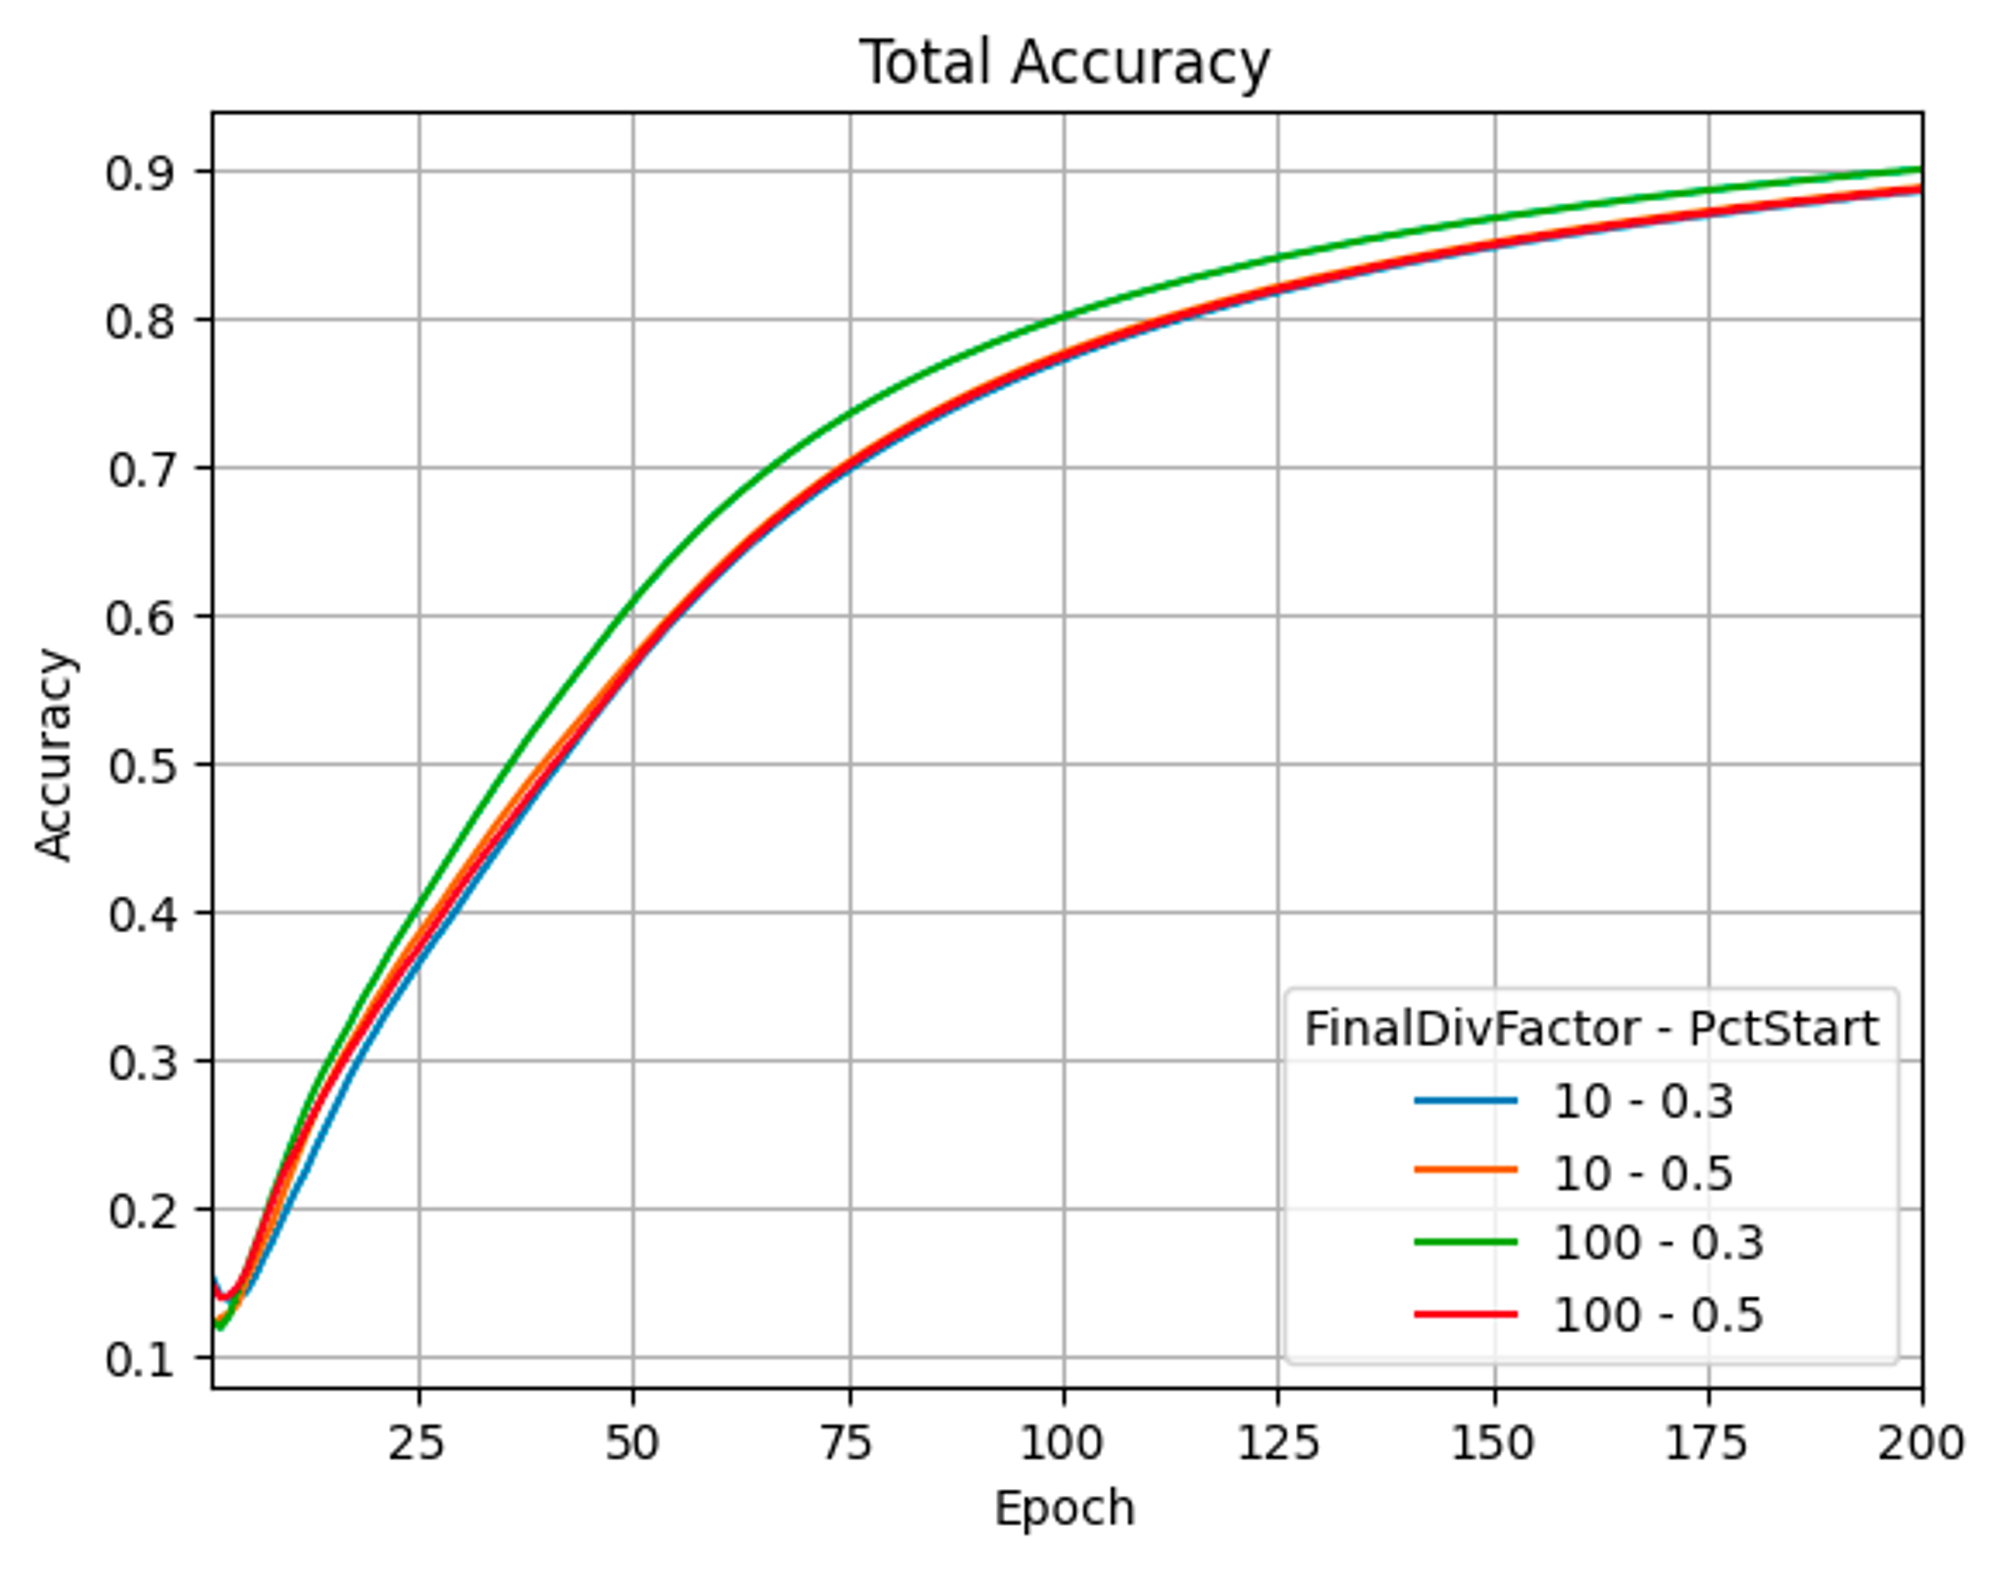
\includegraphics[width=\textwidth]{assets/img/onecycle_tests_train_acc.png}
            \caption{Total accuracy}
            \label{fig:onecycle_tests_train_acc}
        \end{subfigure}%
        \hfill
        \begin{subfigure}[b]{0.3\textwidth}
            \centering
            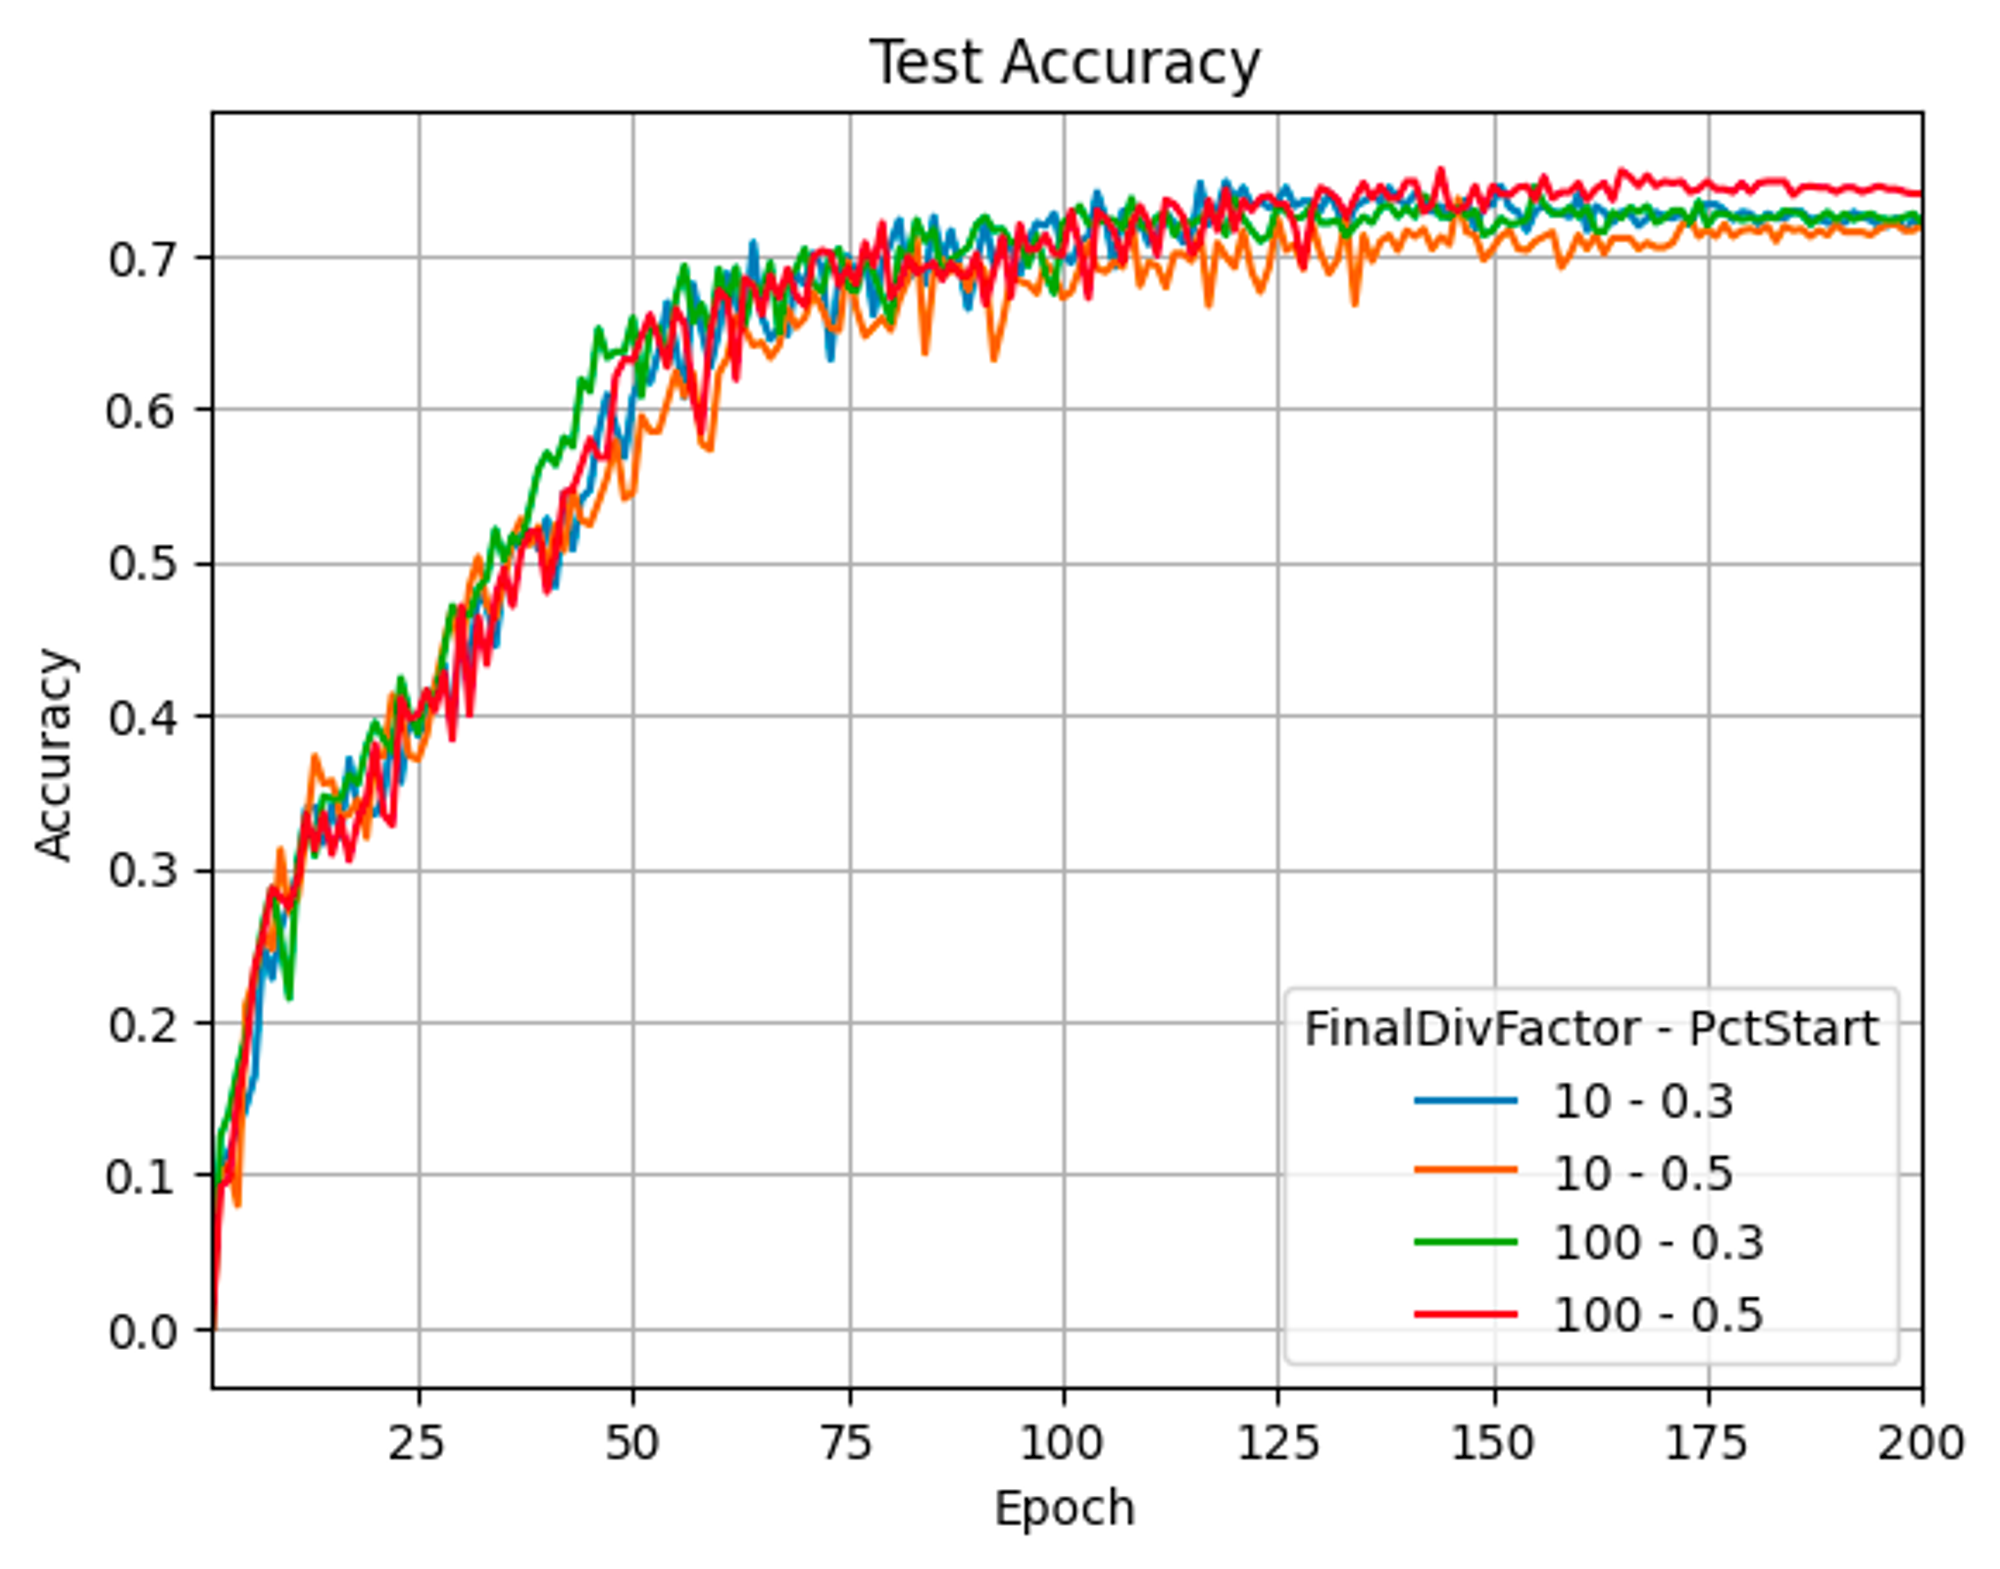
\includegraphics[width=\textwidth]{assets/img/onecycle_tests_test_acc.png}
            \caption{Test accuracy}
            \label{fig:onecycle_tests_test_acc}
        \end{subfigure}%
    \end{figure}

    
\end{itemize}

%%%%%%%%%%%%%%%%%%%%%%%%%%%%%%%%%%%%%%%%%%%%%%%%%%%%%%%%%%%%%%%%%%%%%%%%%%

\chapter{Results and Discussion}
\label{Ch4}
\lhead{Chapter 4. \emph{Results and Discussion}}

\section{Results and Interpretation}
Further tests with the final shown configuration were run. This tests achieved a cumulative train accuracy of 98\% and 95\% and a test accuracy of 78\% and 74\% on a two and ten subject dataset respectively.

The results indicate significant improvements in model performance after reducing the number of channels and selecting specific nodes for analysis. The study also demonstrates the importance of fine-tuning the model as this provided an over 20\% increase in test accuracy after carefully comparing hyper-parameters.

Preprocessing and finding an efficient data structure for the use case was also a big impact in the process as it helped iterate over different inputs, outcomes and selection of data during the research.

\section{Areas of Opportunity}
Some areas of opportunity on this research are as follows:
\begin{itemize}
    \item Test accuracy stagnates after around 120 epochs. This can be either due to the amount of training data or the number of EEG channels being too low.
    \item Low accuracy yielded by the last tests of the model are not suitable for biometric authentication
    \item Classification into N categories may be replaced with 2 categories (Fig. \ref{fig:categories_graphic}). This has the potential to make the model more suitable for identifying a single person.
    \begin{figure}[h]
        \centering
        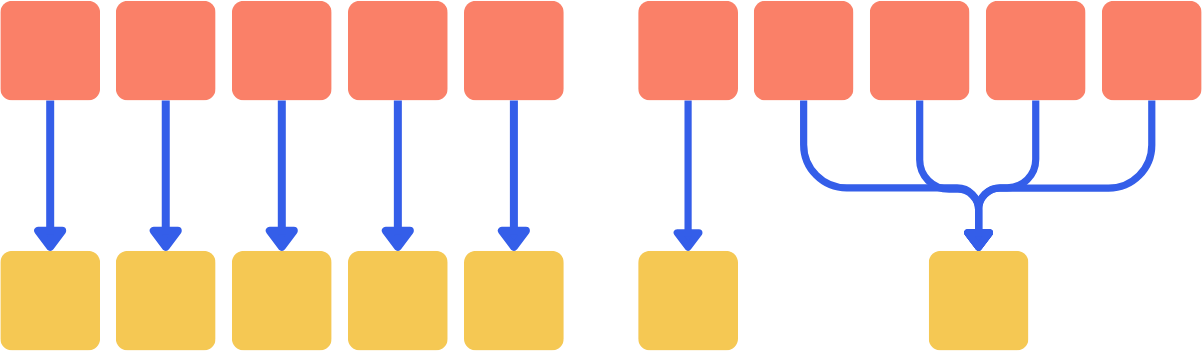
\includegraphics[width=0.6\linewidth]{assets/img/n_to_n_and_n_to_2.png}
        \caption{N to N classification (left) and N to 2 classification (right)}
        \label{fig:categories_graphic}
    \end{figure}
\end{itemize}

\chapter{Conclusions}
\label{Ch5}
\lhead{Chapter 5. \emph{Conclusions}}
In conclusion, this research has resulted in some level of progress in the exploration of brainwave patterns for individual classification through the implementation of Recurrent Neural Networks (RNNs) and the Gated Recurrent Unit (GRU). The challenges associated with low Signal-to-Noise Ratios (SNRs) in multi-electrode setups were acknowledged, prompting the adoption of non-linear techniques, specifically GRUs.

The methodology employed for data selection, preprocessing, and the iterative implementation and fine-tuning of the model has been thoroughly detailed. Key adjustments, including noise reduction through channel selection and the introduction of the OneCycleLR scheduler and Label Smoothing, were instrumental in overcoming obstacles and elevating model accuracy.

The results and discussion section revealed commendable advancements in model performance, with a cumulative train accuracy of 98\% and 95\%, and a test accuracy of 78\% and 74\% on two- and ten-subject datasets, respectively. These outcomes underscore the significance of meticulous fine-tuning efforts and the strategic exploration of hyperparameters.

Areas for future exploration have been identified, particularly the observation of test accuracy plateauing after a specific number of epochs. Further investigation into training data nuances and the potential impact of EEG channels is warranted. Additionally, the suggestion to refine classification into two categories instead of N categories offers potential avenues for enhanced practicality in individual identification.

In summary, the integrative project has significantly contributed to the understanding of applying GRUs to individual classification through EEG signals. The outcomes provide valuable insights for future research, laying the groundwork for continued refinement and ensuring accurate profiling and the development of robust biometric solutions in the future.


%----------------------------------------------------------------------------------------
%	THESIS CONTENT - APPENDICES
%----------------------------------------------------------------------------------------

\addtocontents{toc}{\vspace{2em}}

\appendix 

\chapter{Relevant Code}
\label{AppenA}
\lhead{Appendix A. \emph{Relevant Code}}

% color def
\usepackage{color}
\definecolor{darkred}{rgb}{0.6,0.0,0.0}
\definecolor{darkgreen}{rgb}{0,0.50,0}
\definecolor{lightblue}{rgb}{0.0,0.42,0.91}
\definecolor{orange}{rgb}{0.99,0.48,0.13}
\definecolor{grass}{rgb}{0.18,0.80,0.18}
\definecolor{pink}{rgb}{0.97,0.15,0.45}

% listings
\usepackage{listings}

% General Setting of listings
\lstset{
  aboveskip=1em,
  breaklines=true,
  abovecaptionskip=-6pt,
  captionpos=b,
  escapeinside={\%*}{*)},
  frame=single,
  numbers=left,
  numbersep=15pt,
  numberstyle=\tiny,
}
% 0. Basic Color Theme
\lstdefinestyle{colored}{ %
  basicstyle=\ttfamily,
  backgroundcolor=\color{white},
  commentstyle=\color{green}\itshape,
  keywordstyle=\color{blue}\bfseries\itshape,
  stringstyle=\color{red},
}
% 1. General Python Keywords List
\lstdefinelanguage{PythonPlus}[]{Python}{
  morekeywords=[1]{,as,assert,nonlocal,with,yield,self,True,False,None,} % Python builtin
  morekeywords=[2]{,__init__,__add__,__mul__,__div__,__sub__,__call__,__getitem__,__setitem__,__eq__,__ne__,__nonzero__,__rmul__,__radd__,__repr__,__str__,__get__,__truediv__,__pow__,__name__,__future__,__all__,}, % magic methods
  morekeywords=[3]{,object,type,isinstance,copy,deepcopy,zip,enumerate,reversed,list,set,len,dict,tuple,range,xrange,append,execfile,real,imag,reduce,str,repr,}, % common functions
  morekeywords=[4]{,Exception,NameError,IndexError,SyntaxError,TypeError,ValueError,OverflowError,ZeroDivisionError,}, % errors
  morekeywords=[5]{,ode,fsolve,sqrt,exp,sin,cos,arctan,arctan2,arccos,pi, array,norm,solve,dot,arange,isscalar,max,sum,flatten,shape,reshape,find,any,all,abs,plot,linspace,legend,quad,polyval,polyfit,hstack,concatenate,vstack,column_stack,empty,zeros,ones,rand,vander,grid,pcolor,eig,eigs,eigvals,svd,qr,tan,det,logspace,roll,min,mean,cumsum,cumprod,diff,vectorize,lstsq,cla,eye,xlabel,ylabel,squeeze,}, % numpy / math
}
% 2. New Language based on Python
\lstdefinelanguage{PyBrIM}[]{PythonPlus}{
  emph={d,E,a,Fc28,Fy,Fu,D,des,supplier,Material,Rectangle,PyElmt},
}
% 3. Extended theme
\lstdefinestyle{colorEX}{
  basicstyle=\ttfamily,
  backgroundcolor=\color{white},
  commentstyle=\color{darkgreen}\slshape,
  keywordstyle=\color{blue}\bfseries\itshape,
  keywordstyle=[2]\color{blue}\bfseries,
  keywordstyle=[3]\color{grass},
  keywordstyle=[4]\color{red},
  keywordstyle=[5]\color{orange},
  stringstyle=\color{darkred},
  emphstyle=\color{pink}\underbar,
}
\lstset{style=colorEX}
\lstinputlisting[language=PyBrIM, caption=Data transformation function]{assets/code/data_transformation.py}
\lstinputlisting[language=PyBrIM, caption=GRU definition]{assets/code/gru_definition.py}

The entirety of the code can be found in the GitHub repository:\\
\href{https://github.com/BernardoEstrada/eeg-profiling}{github.com/BernardoEstrada/eeg-profiling}

\addtocontents{toc}{\vspace{2em}}

\backmatter
\label{Bibliography}
\lhead{\emph{Bibliography}}
\bibliography{savedrecs} 
\bibliographystyle{ieeetr}

% \end{bibliography}
%%%%%%%%%%%%%%%%%%%%%%%%%%%%%%%%%%%%%%%%%%%%%%%%%%%%%%%%%%%%%%%%%%%%%%%%%%%%%%%%


\end{document}
